\documentclass[11pt, oneside]{article}   	% use "amsart" instead of "article" for AMSLaTeX format
\usepackage{geometry}                		% See geometry.pdf to learn the layout options. There are lots.
\geometry{letterpaper}                   		% ... or a4paper or a5paper or ... 
%\geometry{landscape}                		% Activate for for rotated page geometry
%\usepackage[parfill]{parskip}    		% Activate to begin paragraphs with an empty line rather than an indent
\usepackage{graphicx}				% Use pdf, png, jpg, or eps§ with pdflatex; use eps in DVI mode
								% TeX will automatically convert eps --> pdf in pdflatex		
\usepackage{amssymb}
\usepackage{hyperref}
\usepackage{listings}
\usepackage{color}
\usepackage[section]{placeins}
\usepackage{graphicx}
\usepackage{caption}
\usepackage{subcaption}
\usepackage{pdfpages}
\usepackage{tabularx}


\definecolor{mygreen}{rgb}{0,0.6,0}
\definecolor{mygray}{rgb}{0.5,0.5,0.5}
\definecolor{mymauve}{rgb}{0.58,0,0.82}

\lstset{ %
  backgroundcolor=\color{white},   % choose the background color; you must add \usepackage{color} or \usepackage{xcolor}
  basicstyle=\footnotesize,        % the size of the fonts that are used for the code
  breakatwhitespace=false,         % sets if automatic breaks should only happen at whitespace
  breaklines=true,                 % sets automatic line breaking
  captionpos=b,                    % sets the caption-position to bottom
  commentstyle=\color{mygreen},    % comment style
  deletekeywords={...},            % if you want to delete keywords from the given language
  escapeinside={\%*}{*)},          % if you want to add LaTeX within your code
  extendedchars=true,              % lets you use non-ASCII characters; for 8-bits encodings only, does not work with UTF-8
  frame=single,                    % adds a frame around the code
  keepspaces=true,                 % keeps spaces in text, useful for keeping indentation of code (possibly needs columns=flexible)
  keywordstyle=\color{blue},       % keyword style
  language=Octave,                 % the language of the code
  otherkeywords={*,...},            % if you want to add more keywords to the set
  numbers=left,                    % where to put the line-numbers; possible values are (none, left, right)
  numbersep=5pt,                   % how far the line-numbers are from the code
  numberstyle=\tiny\color{mygray}, % the style that is used for the line-numbers
  rulecolor=\color{black},         % if not set, the frame-color may be changed on line-breaks within not-black text (e.g. comments (green here))
  showspaces=false,                % show spaces everywhere adding particular underscores; it overrides 'showstringspaces'
  showstringspaces=false,          % underline spaces within strings only
  showtabs=false,                  % show tabs within strings adding particular underscores
  stepnumber=2,                    % the step between two line-numbers. If it's 1, each line will be numbered
  stringstyle=\color{mymauve},     % string literal style
  tabsize=2,                       % sets default tabsize to 2 spaces
  title=\lstname                   % show the filename of files included with \lstinputlisting; also try caption instead of title
}

\title{Mining educational social networks for student performance classification}
\author{Student: Andreu Grimalt Reynes 
\\\\Supervisor: Matthew Yee-King
\\\\Degree: BSc Creative Computing}
\date{}							% Activate to display a given date or no date
\bibliographystyle{plain}

\begin{document}
\maketitle
\newpage
\abstract
\noindent
This document is a report on the study of the relationships between feedback and student performance in the context of Educational Data Mining. Data from an online educational social network was analysed in order to try to find correlations between students' behaviour and final grades. The students' behaviour was characterised with feature vectors to make differentiation and comparison of students possible. The main aim was to find a method that would allow the classification of students from the analysis of log data containing interactions with an educational social network.
Two studies on the data are presented, they experiment with different feature vectors and Data Mining methods: On one hand, a high level data analysis explores the data and calculates various statistics. Plots and linear regressions are calculated which fail to find any correlations between feedback activity and student performance.\\
On the other hand an exploratory data analysis experiments with different feature vectors and Data Mining methods. The methods used to analyse the data belong to the Data Mining field and based in a $k$-nearest neighbour classification, $k$-means clustering and PCA. The method used with $k$-nearest neighbour is able to classify students into performance categories with an accuracy of 0.7980.

\section{Introduction}
In the context of education, assessment is a fundamental aspect of any learning process. An assessment is defined as a ``judgement which can be justified according to a weighted set of goals the result of which is usually a comparative or numerical rating'' \cite{Scriven1967}. The process of assessment consists in the methodology used to produce the judgement and involves testing the student knowledge against a set of weighted learning goals. Assessment in itself is present in most aspects of daily life: A solicitor might assess the chances of winning a case, a doctor might assess the evolution of a patient, etc. However, its effects on education are dramatic: Assessment is not only responsible for rating students' knowledge but it can also play a fundamental role in aiding the learning process. As an example of the role of assessment on the learning process, Bigg's proposes Constructive Alignment as a method to ensure that student activity is focused on the course material by aligning course activities and assessments using learning outcomes \cite{Biggs2002}.\\ 
There are two types of assessment in an educational context: Summative assessment is responsible for producing a grade. It is usually carried out at the end of a course and its aim is to encapsulate students' knowledge in order to measure it (often by examination). Formative assessment is used to aid learning and prepare for a summative assessment. It is generally carried out through a course and it requires feedback. Formative and summative assessment are the same process, the only difference being that formative assessment requires feedback. An example of summative assessment would be a test where students get back a mark without any feedback. On the other hand, an example of formative assessment would be a test where students get back a mark and a justification explaining why they got that grade.\\\\
Formative assessment is fundamental to education nowadays. %and till some point it is a measure of the quality of education. 
It has been adopted by education curricula in most countries, being the preferred choice by education professionals and students. An example of this is the National Student Survey \cite{nationalStudentSurvey}. It is an annual survey taken by higher education students in their final year, the questions relate to formative assessment which shows how feedback is considered fundamental by educational institutions and students alike.\\
A fundamental component of formative assessment is feedback, where students receive a justification of the assessment outcome. The word feedback is present in many different contexts and therefore there are numerous definitions in the literature. Some authors consider feedback to be information about the difference between the actual level of a piece of work and a reference level which is used to alter this gap in some way \cite{Ramaprasad}. Other authors argue that feedback requires knowledge of the goals and skills in making comparisons and suggestions to reduce the gap between what is produced and the goal \cite{Sadler1998}. A definition of feedback from an AI perspective is provided by John Hattie \cite{HattieHelenE-MailAddress2007}: `Feedback is conceptualised as information provided by an agent (e.g., teacher, peer, book, parent, self, experience) regarding aspects of one's performance or understanding. [...] Feedback thus is a consequence of performance'.\\\\
On this project feedback is considered to be the information about the gap between the work produced and the gold standard. %The act of giving feedback requires of the skills to make informed judgements and the experience in transmitting suggestions effectively.
The act of giving feedback requires skills in making informed judgements as well as experience in transmitting suggestions effectively.\\\\
\subsection{Personal experience on feedback in higher education}
My experience in higher education comprises two degrees in different countries with completely different approaches to education. I studied physics in a Spanish university where assessment was almost exclusively summative. The subjects where very similar in content to those of any other university and the material was delivered by a lecturer in weekly sessions. These courses were very structured, at the start of the course the topic to be studied was exposed and in the following sessions the lecturer proceeded with mathematical demonstrations. Each topic was rarely covered in one session, some of them needed months or even a full academic year to cover. The lecturers frequently followed famous text books that contained the different demonstrations. There was no interaction between teacher and students during the lectures, the students were free to ask questions but the atmosphere in the lecture was not usually encouraging. Additionally, the gap between the course content and the knowledge of students was enormous making it very difficult to even be able to ask a question.\\
Apart from theory lectures there were practical sessions that consisted only in the resolution of exercises. The function of these sessions was to provide formative assessment (i.e feedback to students' about their knowledge in the topic) as well as preparation for the final exam. Unfortunately, the exercises were too complicated to even ask questions and the lectures consisted simply in the lecturer resolving problems himself or herself with no interaction with the students who limited to copy form the whiteboard.\\
When I started my physics degree I was fascinated by the subject but over time my interest diminished dramatically. Part of that was the total lack of formative assessment. Assessment was seen as a punishment in spite of just another tool for learning. The summative assessment created the impression that grades were more important than actual learning. There was a point when I realised that I was passing exams with very little knowledge about the subject and I decided to end my studies.\\\\
Most courses I studied at Goldsmiths were assessed with formative assessment. However, some of them had a summative assessment at the end of the course (an exam) that produced the final grade. Following my experience in my previous degree, the type of assessment has a dramatic impact in the engagement I felt towards a topic or a subject. Through formative assessment I felt passionate about learning and more importantly I learned. With summative assessment I felt the need to memorise information -which does not automatically involve learning- in order to write it down efficiently on an exam.\\
My personal experience demonstrates how critical feedback is. When feedback is present I learn, when feedback is not present I disengage and merely memorise. To conclude, I argue that the type of learning experienced following summative assessment is poor as opposed to the rich and fulfilling process of learning through formative assessment.\\\\
% if there's need to stretch all this I can relate to social role of assessment
%This project investigates the effects of feedback in the context of educational social networks. 
\subsection{Online education}
With the popularisation of social networks, the internet has become a repository of information where data is intensively shared, reviewed and discussed by communities of users. One might argue that the internet is commonly used for learning not only by students but also by professionals looking for hints or even complete solutions to problems. If one accepts that life is a constant learning process, then this learning has been accelerated and optimised by the Internet whose role is to facilitate the access to information and allowing for a constant interchange of feedback between people. This type of interaction between humans and machines was described by Tim Berners-Lee in {\it Weaving the Web: The original design and ultimate destiny of the World Wide Web by its inventor} \cite{berners2000weaving} as a system where humans do the creative work and machines do the administrative part. Such a system is called a {\it social machine}. In the context of an educational social machine the creative work would be to provide formative assessment whereas the administrative part would be to provide all the technology and infrastructure for the online course to exist.\\\\
Social networks have provided a new paradigm on education where learning and especially feedback is delivered on the web. This is manifested in how users use popular social network commenting tools (forums and discussion threads) to learn about a particular topic. In some cases users look for straight answers to specific problems, however, on other cases users seem to be `interested' in the topic. This `interest' or engagement is a very interesting phenomena and I argue that it has been maximised by the extensive use and adoption of social networks. It is consistent with the learning achieved through formative assessment where students are engaged with the subject and discussions about topics are spontaneous. It creates communities of learners where ideas are exchanged and reviewed in a process that can be described as giving and receiving feedback.\\ Youtube is arguably one of the most popular social networks that is used for learning. A good example of how this social network is used in an informal educational context is Periodic Videos \cite{PeriodicVideos}. It is a Youtube Channel owned by the University of Nottingham Chemistry Department, it has 2,298 videos about chemistry with a total of 291,658,881 views. Each video has hundreds of comments where a substantial number of them initiate discussions about chemistry. The list of Youtube Channels dedicated to education is immense and it is constantly growing. As pointed out, most of these channels are targeted to non formal learning and most of their popularity and success is probably due to this reason.\\\\
Over the last fifteen years higher education institutions have been transitioning to virtual learning environments (VLE) to support their education services. Universities use systems like Moodle \cite{Moodle} that provide a virtual environment where students and teachers can interact with each other. VLEs typically contain course materials, assignment submission tools and forums where students can engage in discussions among other tools. However, the social potential of the VLEs is often not exploited or used very scarcely. An important detail is that VLEs are usually closed to the public meaning that only students of a particular course (or institution) have access to them.\\\\
The idea of an online course open to anyone on the Internet crystallised in MOOCs (Massive Open Online Courses) \cite{YearOfMooc}. MOOCs are courses produced by major educational institutions that have a high number of students and are free of charge. The content of MOOCs usually consists of video lectures, reading lists and exercises but also in-lecture quizzes and interactive forums to support communities of learners. These types of courses are usually distributed in online platforms offering a wide range of courses from different subjects. MOOC platforms were popularised by three companies: Coursera, edX and Udacity. All three appeared in 2012, a fact that prompted the New York Times to coin 2012 as `The Year of the MOOC' \cite{YearOfMooc}. One can think of these platforms as a new type of `university', they offer different courses on a varied range of subjects from some of the most prestigious educational institutions.\\
One of the issues MOOCs need to address is that the title achieved after successful completion usually lacks any formal academic recognition. In this regard, there is still a long way to go to be able to compare MOOCs with higher education courses.\\
MOOCs provide a privileged platform to encourage a more social and interactive educational experience. As explained above, online forums have been traditionally used as platforms for communities of learners. However, recently there has been a shift towards a type of formative assessment called peer feedback. Peer feedback consists in an interchange of feedback between two students. By using an online peer feedback system students can support each other, express concerns or find solutions to problems collectively. More importantly they can teach and learn together, thus creating communities of learners through feedback and social interaction. Online peer feedback systems allow students to formatively assess each other anytime anywhere.\\\\
We have seen how important the role of feedback is and how formative assessment can be optimised through peer feedback. Additionally, I presented my personal experience on how summative and formative assessments are needed in order to facilitate learning. An interesting question is whether or not it is possible to establish the relation between these two types of assessment, in other words, whether or not it is possible to quantify the effects of feedback on a learning process. In order to measure that magnitude, one needs access to large amounts of data relating to student behaviour, feedback and student performance. %The idea is to combine data mining techniques with pedagogical theory and empirical evidence in order to add some light into this issue. 
The surge in student behaviour data provided by the online systems described above allowed researchers to develop methods to study educational questions. This new emerging field encapsulates multidisciplinary techniques under the name of Educational Data Mining. It consists in the application of Data Mining methods to educational data with the objective of resolving educational research questions.\\
In this project I attempt to use data mining techniques in order to classify student performance from their behavioural patterns after receiving feedback. The data used was generated in a case study involving Music Circle, a social network for learning developed within the PRAISE research project at the computing department at Goldsmiths. The students undertook a creative programming MOOC that run on Coursera \cite{Coursera}. It lasted for six weeks and it was completed by 3,715 users. Students had access to video lectures where theory and exercises were presented. The exercises were audio-visual programming assignments and once completed they had to be screen recorded, uploaded to Vimeo and then submitted to Music Circle for discussion among peer students. Music Circle logs all the mouse events of the users and from the log data it is possible to infer when feedback takes place. In order to classify students into academic performance from their feedback activities, the data from the MOOC assessments (final grades) and the logs in Music Circle is analysed with Data Mining algorithms.

\subsection{Report structure}
The introduction section discusses pedagogical terms such as assessment and feedback, as well as a personal experience in two higher education institutions that had different approaches to assessment. Additionally, it explains how the birth of educational social networks sparked a whole new field called Educational Data Mining which aims to apply Data Mining algorithms to answer educational research questions.\\\\
The background section contains an overview of the methods and papers published in the field of Educational Data Mining, as well as a description of some of the technologies used to analyse the data. An overview of Data Mining and Educational Data Mining is provided, followed by examples of applications of these fields to the analysis of social networks and educational data.\\\\
The Data section contains a description of the data analysed in the project as well as the technologies used to perform the analysis. The different databases are described as well as the processes to build them.\\\\
Section 5 and section 6 contain the two main studies on the data: On one hand, a high level data analysis calculates statistics about the data. The aim of this study was to explore the data and present statistics that would offer clues about how to analyse it. Statistics about social network usage are presented as well as final grades and activity after feedback. On the other hand, an exploratory data analysis experiments with different feature vectors and Data Mining algorithms in order to find correlations between feedback activities and student academic performance.\\\\
The last section contains a reflection on the project as a whole. It compares the project to the initial proposal and tries to explain the causes of divergence. Additionally, it describes the difficulties experienced during the project and it proposes future work in other to continue the research.

\section{Background} 
This section contains an overview of the research about the intersections between data mining and education. It contains a general description about data mining and educational data mining followed by concrete examples on data mining applied to education.
\subsection{Data Mining}
Data mining (DM) is a multidisciplinary subject which aims to discover patterns in very large datasets, it uses algorithms from computer science, artificial intelligence, machine learning and database theory. %Data is generated at increasing rates by the surge of mobile devices and social networks which practically means that very large datasets can be built fast and inexpensively. These large datasets receive the name of `Big Data' and they are the target of Data Mining. Data Mining is used in order to extract knowledge from Big Data. Depending on the nature of the data, the knowledge extracted can be used in a wide range of applications that range from business analysis to medical applications or scientific research.\\\\
\\\\
From a historical point of view Data Mining can be viewed as an evolution of information technology. As with any other technological field, database technologies have been following a rapid expansion over the last fifty years: The limitations of early database systems that allowed primitive file processing prompted the development of database management systems in the early 70s. These systems introduced new paradigms such as hierarchical, network and relational databases, indexing and accessing methods, query languages such as SQL, user interface and finally online transaction processing. In the mid-80s advanced database systems were developed, these systems included advanced data models and they were applied to a wide range of data from engineering to multimedia.\\ 
It is in the late 80s that the design of databases considered the analysis of the data they contained. Data warehouse technology was developed as well as a new field which aimed to extract knowledge from the databases, this new subject was Data Mining. Data Mining continued its growth with the invention of the Internet and it surged with the increase of data driven technologies such as mobile devices and social networks \cite{Han:2005:DMC:1076797}.\\\\
Nowadays, data is generated at increasing rates aided by the popularisation of mobile devices (and sensors) as well as social networks. This situation allows systems to build very large datasets in a fast and inexpensive way. These large datasets are usually referred to as `Big Data' and they are the target of Data Mining. Depending on the nature of the data, the knowledge extracted can be used in a wide range of applications that range from business analysis to medical applications or scientific research.\\\\
%As explained above, data mining aims to discover knowledge that is `hidden' in the data. 
With this knowledge one can build models of the data and then use those models to classify data instances or make predictions. Two of the main problems in Data Mining are classification and regression. A regression problem is focused in producing a value whereas a classification problem is focused on assigning classes to data instances.\\\\
According to Jiawei Han the Data Mining process contains the following steps \cite{Han:2005:DMC:1076797}:
\begin{itemize}
	\item Data cleaning: Removal of any noise or inconsistent data
	\item Data integration: Combination of multiple data sources
	\item Data selection: Retrieval of relevant data from the database
	\item Data transformation: Consolidation of data into appropriate forms for mining
	\item Data mining: Application of algorithms to extract knowledge
	\item Pattern evaluation: Identification of interesting patters using metrics
	\item Knowledge presentation: Presentation of results
\end{itemize}

\subsection{Data preparation}
A crucial task on Data Mining is the preparation of the data for analysis, a process also known as data pre-processing. The databases used for DM are large, often in the Gigabytes order of magnitude. Such systems are complex and the data sources are often heterogeneous which results in data being noisy, missing or inconsistent. Data with those features has low quality, meaning that DM algorithms will produce poor results when using it. Therefore, the aim of data pre-processing is to improve the quality of the data so that DM algorithms produce useful results.\\
Different techniques have been proposed to improve the quality of the data: Data cleaning minimises noise and corrects inconsistencies. Data integration combines data from different sources creating a coherent database. Data transformation manipulates the data by finding representations that maximise its potential. Finally, data reduction selects the most important features of the data thus reducing its size, increasing processing speed and improving the results.\\\\
Data cleaning techniques focus on filling gaps in the data, smoothing values and correcting inconsistencies. Several options are available when dealing with missing values: 
\begin{itemize}
	\item Remove the tuple: If one component of the tuple is missing, then discard the sample
	\item Filling the missing value manually: This approach is time consuming and not feasible for large datasets
	\item Use a constant: When a missing value is encountered, then substitute it for a constant value
	\item Use the attribute mean: Calculate the mean of the attribute considering all samples and substitute by that value
	\item Use the most probable value: Use machine learning algorithms to predict the value
\end{itemize}
Noise is a random error or variance in the data. These are several techniques that can help to minimise noise:
\begin{itemize}
	\item Binning: These methods smooth the data by comparing it with similar samples which are grouped into bins. The samples' values are substituted by the bin mean, bin median or bin boundaries
	\item Regression: The data is fitted to a function and sample values are substituted by the output of the fitted function
	\item Clustering: Clustering is an effective way of detecting outliers. Any sample that does not fall into a cluster is eliminated. 
\end{itemize}
Data integration consists in merging data from various sources in order to produce a coherent database that can be used by DM algorithms. As an example consider a system that uses a database to perform its operations. The database of such a system will be optimised for the retrieval and modification of data according to that particular system. That database might not be ideal to perform data mining operations, therefore, a new database can be created which will contain the system's data stored in a way that makes it efficient for DM algorithms.\\\\
Data transformation aims to transform and consolidate the data into appropriate representations for mining. Some of the common methods for data transformation are:
\begin{itemize}
	\item Smoothing: Remove noise from data with the techniques described above
	\item Aggregation: Similar to data integration
	\item Generalisation: Low-level values are replaced by high-level attributes
	\item Normalisation: Scale the data between [-1,1] or [0,1]
	\item Attribute construction: Generation of new features from the given set of attributes
\end{itemize}
Data reduction aims to find a representation of the data that is smaller in size but retains the basic properties of the original data set. That means that DM on the reduced data set produces similar results yet increasing the processing speed.\\\\ 
One of the most common data reduction techniques is Principal Components Analysis (PCA). Given a set of $k$-dimensional vectors, the aim of PCA is to find $n$ orthonormal vectors where $n<k$, the dimension of the vector space is reduced thus allowing to represent the data set into a dimensional smaller space. PCA is an orthogonal transformation that transforms a possibly correlated set of vectors into a linearly uncorrelated vectors called principle components. These principal components are sorted in a decreasing variance value. The principal components then represent a new set of axes that contain information about the variance of the data. PCA combines attributes from the different vector to create a smaller representation of the data that usually reveal dependancies that were not trivial.

\subsection{Eduational Data Mining}
Educational Data Mining (EDM) is an emerging discipline that aims to apply data mining techniques to educational data in order to answer questions about educational research \cite{EDM}.
``EDM is concerned in the development of methods for making discoveries within the unique kinds of data that come from educational settings, and using those methods to better understand students and the settings which they learn in'' \cite{Baker2010}. The increasing use of the Internet for education and the development of online education systems generates large datasets that contain information about teacher-student and student-student interaction. The aim of EDM is to use these datasets to better understand the learning process and to develop systems that optimise the learning experience.\\
C. Romero and S. Ventura identify three main research areas in EDM \cite{Romero2010}:
\begin{itemize}
	\item Offline education that transmits knowledge through in-person interaction and tries to understand how humans learn. It borrows from psychometrics and it applies statistical techniques to data gathered in classroom environments. 
	\item E-learning and Learning Management Systems are new educational platforms that deliver their content through the Internet. They intend to be a virtual environment that emulates the traditional teaching setting.
	\item Intelligent Tutoring and Adaptive Educational Hypermedia System are systems that focus on the optimisation of the learning experience on the web therefore providing a system that adapts to every student needs. This systems tend to generate vast amounts of data such as log files or user models that can be analysed using DM algorithms.
\end{itemize}
Authors suggest many areas in the application for EDM \cite{Castro2007},\cite{Baker2010},\cite{Romero2010}. These applications use traditional DM techniques such as classification, clustering and association rules but also other methods that are not exclusively considered DM such as visualisation and regression.\\
The analysis and visualisation of data highlights useful information and supports decision making. It can be used to analyse students activities to provide a general view of a course. The techniques used in this task are statistics and data visualisation. Statistics provide the analysis of the data whereas the visualisation aids the interpretation of it.\\
Feedback for supporting instructors suggest actions for teachers or course administrators that would optimise the learning experience. Association rules are the most common DM technique used for this task. Association rule algorithms find relationships between data in large datasets presenting them as strong rules according to metrics measuring how interesting they are \cite{Piatetsky-Shapiro1991}.\\
Another interesting EDM task is to build a system that makes direct recommendations to students thus offering personalised learning. The most commonly used DM techniques in this case are association rules, clustering and sequential pattern mining.\\
Predicting student performance consists in the estimation of an unknown variable that describes the student (knowledge, score, grade, etc.). This value can be continuous (regression task) or a categorical attribute (classification task). Regression analysis finds the relationship between a dependant set of variables whereas classification assigns classes to individual items based on quantitative information regarding items' features. Some of the DM techniques used for this task are: Neural networks, Bayesian networks, rule-based systems, regression and correlation analysis. % Add more stuff here, it's the most important point \\

\subsection{Analysis of user activity in social networks}
The ubiquitous use of social networks in recent years has sparked research about how to analyse their users behaviour. Traditional methods in the characterisation of user behaviour are not suitable in the online context where users interact with a website, an application or other users through interfaces that implement the social network functionality.\\
As seen above social networks generate large amounts of data regarding user behaviour. However, usually this data is in its raw form and it does not by itself show features useful for an analysis process. Generally the data comes from log files that capture user events or explicit activity that happens on the social network meaning that in order to extract useful knowledge from the data one needs to use DM methods.\\
Unfortunately, DM does not perform well when applied to raw data. The data needs to be reduced in a way that expresses desired features, the features relating to the same item are put together in a vector which is fed to DM algorithms. The process of obtaining features from the raw data is not trivial and it makes up for most of the pre-processing stage in a DM analysis.\\\\ 
Maia and Almeida \cite{Maia2008} propose a methodology for characterising and identifying user behaviours in online social networks. First, they crawled data from YouTube and used a clustering algorithm to group users that share similar behavioural patterns. Next, they showed that attributes that stem from the user social interactions, in contrast to attributes relative to each individual user, are good discriminators and allow the identification of relevant user behaviours. Finally, they present and discuss experimental results of the use of proposed methodology.\\
Of particular interest is a section describing their methods to build feature vectors that allow to discriminate between users. Each user was assigned a nine dimensional feature vector containing features unique to the user but also features about the interaction with other users. The features uniquely relating to a user are: Number of uploads, number of views, number of channel views, system join date and age. The features relating to a community of users are: Clustering coefficient, reciprocity, out-degree and in-degree. The clustering coefficient measure the interconnection between users and their neighbours. The reciprocity measures the probability of mutual subscriptions. The out-degree is the number of subscriptions made by the user and finally the in-degree is the number of subscriptions received by the user.\\
Once the feature vector is constructed it is normalised to allow for the features to have comparable weights. The authors then apply a k-means algorithm to the set of feature vectors, similar users cluster together forming groups thus manifesting different types of users.

\subsection{Analysis of student behaviour in educational systems}
We have seen an example on how feature vectors can be used to characterise user behaviour in social networks. One of the most interesting aspects of EDM is that there is not yet formal methods to analyse student behaviour, this meaning that the methods to obtain feature vectors out of educational data are not well defined.\\
Baker \cite{Baker2012} presented models which can detect student engaged concentration, confusion, frustration, and boredom solely from students' interactions within a Cognitive Tutor for Algebra. ``These detectors were designed to operate solely on the information available through students' semantic actions within the interface, making these detectors applicable both for driving interventions and for labelling existing log files in the PSLC DataShop, facilitating future discovery with models analyses at scale'' \cite{Baker2012}.\\\\
The data collected consisted in log files from the tutoring system and field observation of students behaviour. The log files contained the interaction of students with the interface whereas the filed observation consisted in judgement of the students' state or behaviour on the work context, actions, utterances, facial expressions, body language, and interactions with teachers or fellow students. At the time of analysis the log file data and the filed observations were synchronised and the features were extracted. A total of 232 features were extracted from the data for each student, these features fell into four categories showed in Table \ref{table:BakerTable}. 
\\\\Each vector contained 232 features. In order to optimise the results, these features were selected (also known as feature reduction) using forward selection, where the feature that most improves model goodness is added repeatedly until adding additional features no longer improves model goodness. Once the dimensional reduction was applied to the feature vectors, these were fed into DM algorithms which included J48 decision trees, step regression, JRip, Na\"{i}ve Bayes, and REP-Trees.\\\
The results obtained were better than chance but left room for improvement. Different algorithms performed better depending on the category. For engaged concentration, the best algorithm was K*. For confusion, the best algorithm was JRip. For frustration, the best algorithm was REPTree. Finally, for boredom, the best algorithm was Na\"{i}ve Bayes.
\begin{table}[h!]
	\begin{tabularx}{\linewidth}{|X|X|X|}
		\hline
		 \textbf{Category} & \textbf{Feature} \\ \hline
		 Engaged concentration & Minimum number of previous incorrect actions \\ \hline
		 Boredom & Average time the student took to respond \\ \hline
		 Confusion & Percentage of actions taking longer than 5 seconds after incorrect answers \\ \hline
		 Frustration & Percentage of past actions on the skills involved that were incorrect \\ \hline

	\end{tabularx}
		 	\caption{Categories with examples of features from \cite{Baker2012}}
	\label{table:BakerTable}
\end{table}

\subsection{Prediction of student performance in online discussion systems}
One of the oldest applications of EDM is to predict students performance based on other information that relates to the learning experience of the student. This is a difficult problem to solve since the performance of a student is influenced by a large number of variables that are difficult to control such as socio-economical background or psychological profile. Authors in \cite{Romero2013} proposed the use of different data mining approaches for improving prediction of students' final performance from quantitative and qualitative participation indicators in social network forums. Their objective was to determine how the selection of instances and attributes, the use of different classification algorithms and the date when data was gathered affected the accuracy and comprehensibility of the prediction. Depending on the variable to be predicted one must use one technique or another: On one hand, classification algorithms are useful when the students performance can be described with a categorical value. On the other hand, regression provides a method to assign a numerical value to the predicted performance. Additionally, one can use a density estimator in order to obtain a probability function of the output variable. An important detail might be to notice that most of the research in EDM focus on higher education or university students and more specifically to e-learning. It is this later online systems that provide us with huge amounts of data regarding student behaviour which is valuable to solve this type of problem. Various publications investigate the link between the use of online discussion systems and student performance finding that it is a strong indicator of student performance. In general, these publications analyse both quantitative or qualitative features independently but not in conjunction.\\ 
On his paper, Romero \cite{Romero2013} describes the prediction of students' performance based on quantitative, qualitative and social network information about forum usage by using classification algorithms and clustering.\\\\
The data was gathered from Moodle \cite{Moodle} forums by developing a special module that allowed an instructor to obtain a summary of the activity. The instructor had to grade each of the forum messages according to metrics that measured the degree of online participation. The quantitative indicators were: Number of messages, threads, words, sentences, reads and time. Qualitative indicators consisted in an average score of all the messages sent by each student, the degree of centrality, the degree of prestige and the final mark. The feature vectors contained both the quantitative and qualitative indicators.\\\\
The next step was to pre-process the data by performing instance selection where only a subset of instances was selected, attribute selection (feature reduction) where the dimensionality of the problem was reduced in order to ease the calculations and finally perform data transformation that converted data to an appropriate input format for the DM algorithms.\\
In this study the authors were interested in categorising the students into two classes: Fail and pass. Therefore, this was a classification problem as opposed to a regression problem. Two data mining methods were proposed: On one hand, they proposed to use a traditional classification method since it is the standard DM approach to classification problems. On the other hand, they propose clustering as an alternative method.\\\
The authors then compare all the different algorithms against performance metrics and conclude that EM (Expectation Maximisation) clustering algorithm provides the best result.

\section{Data and databases}
\subsection{Music Circle}
Music Circle is an educational social network developed within the PRAISE research project at the Goldsmiths University Computing Department \cite{Yee-king}. The aim of Music Circle is to allow communities of students to learn online together by providing an online environment with specific tools to give and receive feedback. Music Circle was designed considering the fundamental role of feedback in learning. In the introduction and background sections we saw the dependancies between assessment, feedback, student performance and learning. Additionally, we saw how valuable is the data generated by students using online systems. Music Circle was designed thinking in the collection of student data for posterior EDM analysis. The content of Music Circle is time based media that users can upload. This media can be content generated by the user such as an audio or video recording, or content shared from other social networks such as Youtube or Vimeo. Once the content is uploaded, users can share it with different communities. Once a media item is shared in a community, it becomes visible to all the members of the community and they can start discussions about it.\\\\ 
Music Circle is a web service, meaning that it is formed by two systems: The server-side software interfaces with the database in order to insert, update or retrieve items. The client side is a Javascript web application that implements all the functionality of Music Circle. The server-side and the client-side are connected with a RESTful API. Figure \ref{table:musicCircle} shows the Music Circle web application.
\begin{figure}[h!]
  \centering
    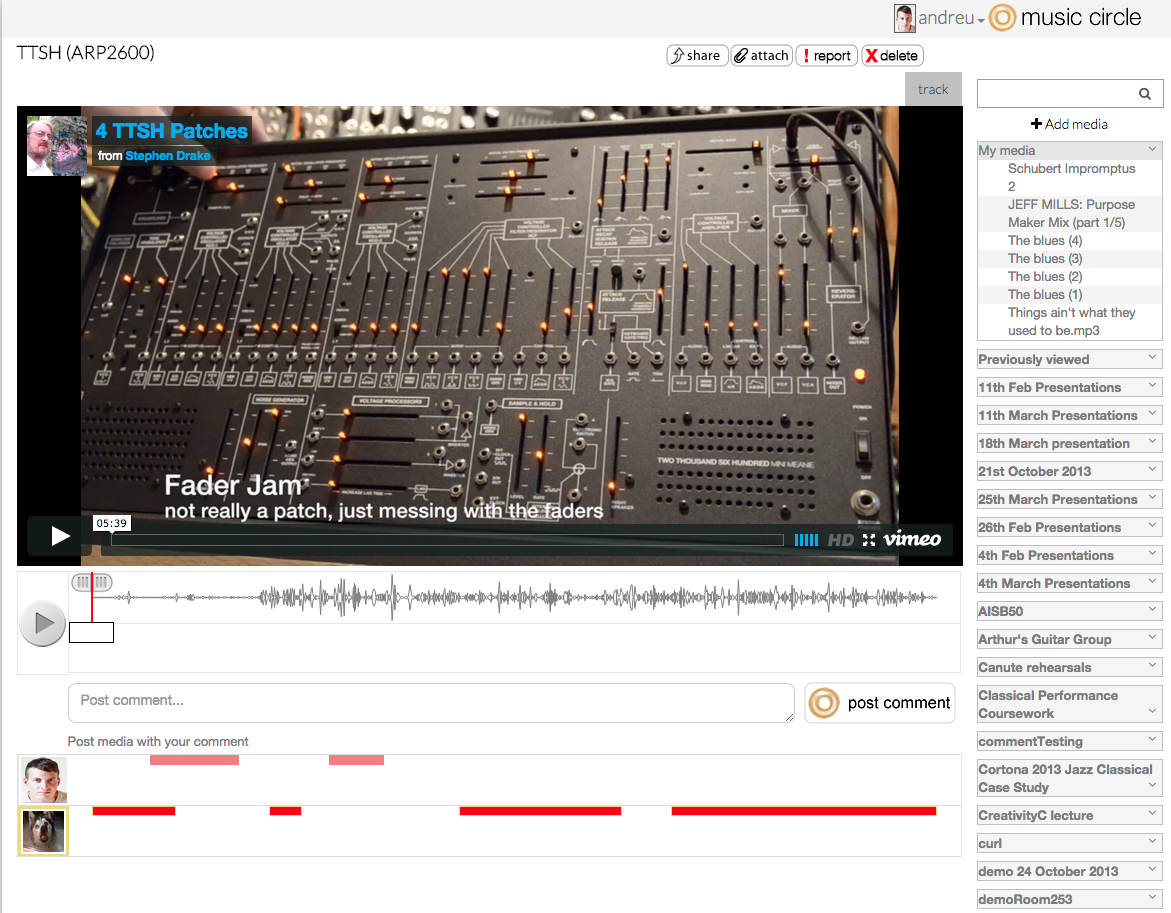
\includegraphics[width=0.6\textwidth]{./musicCircle.png}
      \caption{Music Circle web application}
      \label{table:musicCircle}
\end{figure}
\newpage
\noindent The tool that allows for the discussion of media is the social timeline and it sits at the core of the social network functionality. Using the social timeline, users can select a time region of the media and attach text comments or other media comments to that particular region. Commented regions become can become threaded discussions by adding replies to comments. The selected regions appear as coloured blocks next to the avatar of the user, figure x shows Music Circle's main screen. The coloured blocks represent the time regions selected that have been annotated. Comments that relate to the same region stack on the top of each other, additionally, comment from different users are stacked in layers, thus differentiated by vertical position and colour.\\\\
The data generated by Music Circle consists in the logs generated by the user events when uploading, viewing, commenting and replying. The data has quantitative and qualitative features. On this project only quantitative measures are used, however, it would be interesting to use a qualitative study on the data on future studies. The log data consists in the events generated by the students using the interface and it is described in detail below.\\\\
\subsection{MongoDB}
Traditional databases store the data according to a relational model where the data is separated into tables that represent the different attributes. Data instances are stored in rows that have a unique key. Relations between tables are possible by storing the unique keys that relate to other tables. The relational model of data is very popular and many database technologies make use of it. The structure of the database is defined on creation, therefore, relational databases are not not suitable for data that changes its structure frequently.\\\\
MusicCircle uses a MongoDB database. MongoDB is a document oriented database that provides high performance, high availability, and easy scalability \cite{MongoIntro}.
Document oriented databases rely on the internal structure of the data to infer type information and store all the related information together allowing instances to be different from each other.\\
A MongoDB system can contain several databases. Each of these databases contains a set of collections. The collections hold a set of documents. Documents are at the core of the database and they are the object that stores the data. They are set of key-value pairs and have a dynamic schema that allow documents in the same collection to have different structure or different types of data. In a document, data is stored in BSON (Binary JSON) serialisation format which consists in a binary representation of JSON objects. Therefore, the language used to define documents is JSON and MongoDB language translates it to BSON. The maximum size of a document is 16 megabytes.\\
The queries in MongoDB imply the use of the find() method with a number of query operators in order to select documents from the collections. The query operators consist in exact equality matches and conditionals.\\
MongoDB true power shows in cluster servers where high performance is needed. Replica sets provide high performance replication with automated failover, while sharded clusters make it possible to partition large data sets over many machines.\\\\

\subsection{Databases}
Three different databases were used for this project: Music Circle, Coursera and Research databases. Music Circle contains the data from the Music Circle system, Coursera contains the data from the MOOC that run on Coursera and Research contains a combination of data in Music Circle and Coursera.

\subsection{Coursera}
The Coursera database is a MySQL database that contains the full Coursera course. Of special interest are the tables that contain grades from students. These tables contain the final grades, as well as the multiple choice questionnaires and peer assessment results. Table \ref{table:courseraDatabase} show the relevant tables on the Coursera database.
\begin{table}[h!]
	\centering
	\begin{tabularx}{\linewidth}{|X|X|}
		\hline
		 \textbf{Table} & \textbf{Description}\\ \hline
		 course\_grades & Students final grades \\ \hline
		 hg\_assessment\_evaluation\_metadata & Grades of individual assessments \\ \hline
		 hg\_assessment\_overall\_evaluation\_metadata & Summary of all the grades (final and peer grades) \\ \hline
		 quiz\_submission\_metadata & Multiple choice questionaries results \\ \hline
	\end{tabularx}
	\caption{Coursera database tables that contain students grades}
	\label{table:courseraDatabase}
\end{table}
\clearpage
\subsection{Music Circle database}
The Music Circle database is the one that sits on the server and relates to the web application. It is responsible for storing and serving the data in order to allow the Music Circle clients to work. The database is 19.24 Gb in size and summary of its collections is described in Table \ref{table:musicCircleDatabase}.

\begin{table}[h]
	\centering
	\begin{tabularx}{\linewidth}{|X|X|}
		\hline
		 \textbf{Collection} & \textbf{Description}\\ \hline
		 Activity & Replies \\ \hline
		 ActivityDefinition & Comments \\ \hline
		 ActivityDefinitionTagLinker & Comment tags \\ \hline
		 ActivityDefinitionTagLinker & Reply tags \\ \hline
		 ActivityDefinitionTagLinker & Comments tags \\ \hline
		 aggLeastCommened & List of least commented items \\ \hline
		 aggMostCommented & List of mosts commented items \\ \hline
		 AudioContent & Media Items \\ \hline
		 AudioContentTrackSetLinker &Track sets \\ \hline
		 DeletedComments & Deleted comments \\ \hline
		 DeletedReplies & Deleted replies \\ \hline
		 GenericContent & Files attached to media items \\ \hline
		 log & Log data generated by users events \\ \hline
		 MediaViewLog & Log data generated by users events when watching media \\ \hline
		 Opinion & Rating assigned to a media item, a comment or a reply\\ \hline
		 PraiseUser & User \\ \hline
		 PraiseUserActivityDefinitionStatus & Indicates if a user has not read all the comments \\ \hline
		 PraiseUserAudioContentStatus & Indicates if a user has not played all the media items \\ \hline
		 Session & User session data \\ \hline
		 Tag & Tags \\ \hline
		 TrackSet & Media items set \\ \hline
		 UserGroup & Group of users \\ \hline
	\end{tabularx}
	\caption{Music Circle collections with a brief description of the data they contain}
	\label{table:musicCircleDatabase}
\end{table}

\subsection{Research database}
The Music Circle database was built in order to serve data to the different clients. However, the schema of the database is not optimal for performing Data Mining on its data, therefore, a research database was built considering the analysis of the data. The research database contains documents that relate users with their actions and their items, in this sense, the user field allows every element in the database to be unique.\\\\ 
The user field contains an id in order to make it possible to link with the Music Circle database.\\ 
The activities field is equivalent to the log data in the Music Circle database, it contains the type of activity, the id the element that the activity took place on and a timestamp when it happened.\\ 
The media field contains all the media items for all the users.\\ 
The id filed contains the media item id. The fmt field is the media item format. The owner filed is the user id.\\ 
The title is the title of the media item. The ts filed is the timestamp when the file was uploaded.\\\\
The schema of the research database is presented below, it has three collections: The Actors collection contains users and their actions, the Media collection contains all the media items on the system and the ActorGrades collection contains the users' final grades from the Coursera database.
\begin{verbatim}

    Actors: [
        {
            _id: element id,
            activities: [
                {
                    at: activity type 
                    id: id of the element the action took place on,
                    ts: timestamp
                }
            ],
            sessions:[
            	{
		    logged_in': 1 if used was previously logged in, 
		    sessionID: session id, 
		    sessionStart: date at which the session started, 
		    user_id: user id
		}
            ],
            idx: user id on the Music Circle database,
            name: name oft heuser,
            
        }
    ],
    ActorsGrades: [
         {
              _id: element id,
              id: actor id,
              grade: final grade
         }
    ],
    Media: [
        {
            _id: element id,
            fmt: media format,
            owner: userid,
            title: title of the media item,
            ts: timestamp,
         }
     ]
    \end{verbatim}
The possible values for `at' are: 0=upload, 1=view, 2=comment, 3=reply, 4=login, 5=play, 6=log data (mouse events) whereas the possible values for `fmt' are: 0=video, 1=audio.\\\\
This schema was initially proposed by Dr. Chris Kiefer who previously did research on the same dataset and it was adapted on this project to accommodate all the data needed for the particular studies.\\\\
To build the research database was difficult. The process of importing the data from the Music Circle database into the Research database consisted in iterating through various of the collections in the Music Circle database, putting the data in the right format and inserting it into the right element in the research database. This process is performed by script [\ref{importScript}] and described in detail below:\\
The PraiseUsers collection is iterated and for every user a new document is inserted into the Actions collection which contain the user id, the username and an empty activities array. Figure \ref{figure:praiseUserImport} illustrates the process.
\begin{figure}[h!]
  \centering
    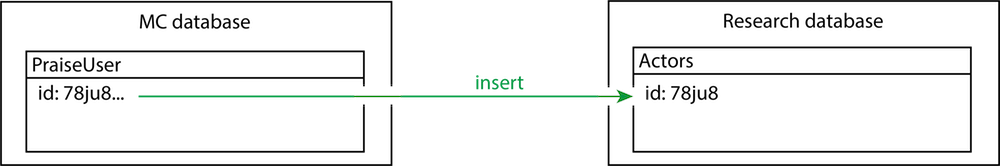
\includegraphics[width=0.6\textwidth]{./praiseUser.png}
      \caption{Import users into the research database}
      \label{figure:praiseUserImport}
\end{figure}
\newpage
\noindent
The AudioContent collection is iterated and for every media item a new document is inserted into the Media collection which contain the media id, the media format, the user id that owns the media item, the title of the media item and a timestamp. Figure \ref{figure:media} illustrates this process.
\begin{figure}[h]
  \centering
    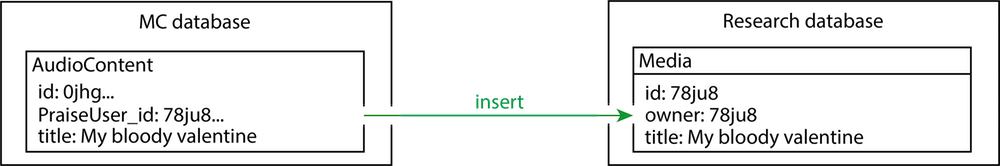
\includegraphics[width=0.6\textwidth]{./media.png}
      \caption{Import media items into the research database}
      \label{figure:media}
\end{figure}
\\The ActivityDefinition collection is iterated and a new object is built which contains the type of activity (comment activity in this case), the id of the comment, the timestamp when it happened, the media item id it belongs to and the text of the comment. The user id of the owner of the comment is known and it is used to find the document for that particular user in the Actors collection. The object previously built is then pushed into the activities array in the correct element on the Actors collection. Figure \ref{figure:activityDefinition} illustrates this process.
\begin{figure}[h!]
  \centering
    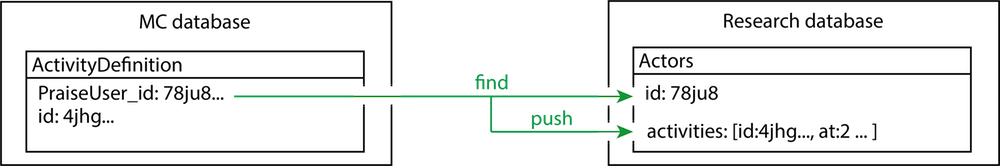
\includegraphics[width=0.6\textwidth]{./activityDefinition.png}
      \caption{Import comments into the research database}
      \label{figure:activityDefinition}
\end{figure}
\\The Activities collection is iterated and for each reply a new object is built which contains the type of activity (reply in this case), the id of the activity, the timestamp when it happened and the comment id it belongs to. The user id of the owner of the reply is known and it is used to find the document for that particular user in the Actors collection. The object previously built is then pushed into the activities array in the correct element on the Actors collection. Figure \ref{figure:activity} illustrates this process.
\begin{figure}[h!]
  \centering
    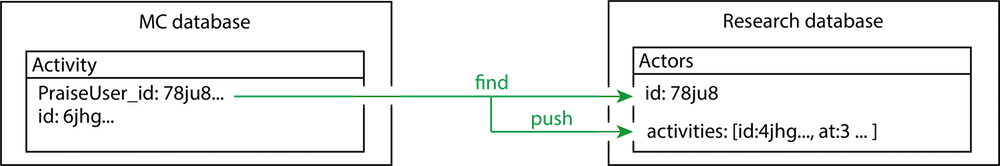
\includegraphics[width=0.6\textwidth]{./activity.png}
      \caption{Import replies into the research database}
      \label{figure:activity}
\end{figure}
\\The MediaViewLog collection is iterated and for every log element a new object is built which contains the type of activity (media view in this case), the timestamp when it happened and the id of the media item that the user viewed. The user id of the owner of the reply is known and it is used to find the document for that particular user in the Actors collection. The object previously built is then pushed into the activities array in the correct element on the Actors collection. Figure \ref{figure:mediaViewLog} illustrates the process.
\begin{figure}[h!]
  \centering
    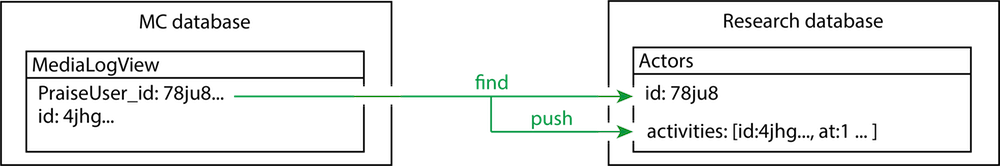
\includegraphics[width=0.6\textwidth]{./mediaLogView.png}
      \caption{Import media view logs into the research database}
      \label{figure:mediaViewLog}
\end{figure}
\\The Sessions collection is iterated and for each session a new object is built which contains the type of activity (logging in) and the timestamp when it happened. The user id of the owner of the reply is known and it is used to find the document for that particular user in the Actors collection. The object previously built is then pushed into the activities array in the correct element on the Actors collection. Figure \ref{figure:sessions} illustrates the process.
\begin{figure}[h!]
  \centering
    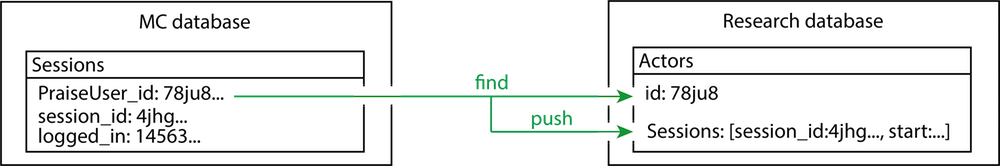
\includegraphics[width=0.6\textwidth]{./sessions.png}
      \caption{Import sessions into the research database}
      \label{figure:sessions}
\end{figure}
\\Finally, the log collection is iterated and its data is imported. Figure \ref{figure:logImport} illustrates the process.
\begin{figure}[h!]
  \centering
    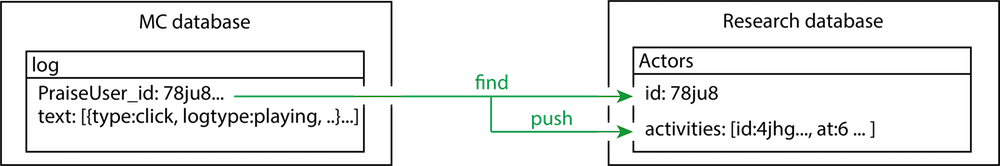
\includegraphics[width=0.6\textwidth]{./log.png}
      \caption{Import logs into the research database}
      \label{figure:logImport}
\end{figure}
\\The log collection is the largest one in the Music Circle database and contains mouse user events from the usage of the Music Circle web client. The size of this collection means that it is not possible to use the approach to import the data described above since it takes a lot of time. When the simple method (the one from above) was tried, the script ran on the machine for two days having completed only a quarter of the collection size. The nature of the log data also meant that it was difficult to predict how much time it would take for the import to complete. The size of individual elements in the log collection varies greatly, meaning that the speed at which the data was imported into the research database was not constant.\\
One of the approaches to try to lower the importing time was to process the data in batches. This way, the amount of data to be processed was low and in theory the computational speed faster. However, the process that slowed down the importing was to update the activities arrays and specially pushing elements at the end of them. Unfortunately, batch processing did not increase the computational speed enough. After this, bulk operations were tested. Bulk operations are standard in Mongo and allow to do a large number of operation in an optimised way, unfortunately it did not work either.\\
When the Mongo process was inspected it showed a CPU usage close to 100\%. Considering that the machine used contained 4 CPUs, it was clear that by using parallel computing the importing speed could be increased dramatically (at least by a factor of 4). For this to happen, the research database had to become a distributed system that allowed multiple Mongo instances running in subsets of the data, this approach would allow the maximisation of CPU usage.
\subsubsection{Scaling of distributed systems}
Two common techniques to scale distributed systems are vertical scaling and sharding:
Vertical scaling consists in adding more CPU and storage resources to increase capacity. Scaling by adding capacity has limitations: high performance systems with large numbers of CPUs and large amount of RAM are disproportionately more expensive than smaller systems.\\
Mongo response to distributed systems is sharding also known as horizontal scaling. It consists in dividing and distributing the data over multiple servers or shards. Each shard is an independent database, and collectively, the shards make up a single logical database. Sharding addresses the challenge of scaling to support high throughput and large data sets:
Sharding reduces the number of operations each shard handles. Each shard processes fewer operations as the cluster grows. As a result, a cluster can increase capacity and throughput horizontally.
For example, to insert data, the application only needs to access the shard responsible for that record.
Sharding reduces the amount of data that each server needs to store. Each shard stores less data as the cluster grows.
For example, if a database has a 1 terabyte data set, and there are 4 shards, then each shard might hold only 256GB of data. If there are 40 shards, then each shard might hold only 25GB of data.\\
Mongo supports the sharding of databases through the configuration of a sharded clusters. A sharded cluster contains these elements: Query routers, config servers and shards (see Figure \ref{figure:datapipeline}).\\
In a sharded cluster, Mongo clients connect to the query routers and these redirect the queries to the appropriate shards. The query router targets operations to the shards and then returns the results to the clients. In real world deployments of sharded clusters there are more than one query router in order to balance the request load even though a particular client sends queries to only one query router at a time.\\
Config servers contain the cluster metadata. They contain a mapping between the clusters data and the shards and the query routers use this metadata to target the shards. A Mongo sharded cluster contains exactly three config servers.\\
Shards are the structures that store the data. In a Mongo sharding the data gets distributed at a collection level, that is to say that the shards will contain data from a particular collection. The distribution of the data is controlled with a shard key. A shard key is either an indexed field or an indexed compound field that exists in every document in the collection. MongoDB divides the shard key values into chunks and distributes the chunks evenly across the shards. To divide the shard key values into chunks, MongoDB uses either range based partitioning or hash based partitioning. Mongo manages the distribution of chunks in the different shards. Chunks are split when they grow beyond a set chunk size and migrates them when a shard contains too many chunks compared with the other shards.\\\\
The sharded cluster built for the Research database had four shards that allowed the four CPUs of the machine to be used simultaneously. Importing the log data using a sharded cluster took 12 hours.\\\\ 
The process to import the log collection is described here: The log collection was processed in batches containing log data between two particular dates. There were four clients connected to the query router, each one importing data from a partition of time (usually two weeks). For each fraction of time, the log collection was iterated. Each element in the log collection is an object containing a user id and a set of logs corresponding to that user. The set of logs is iterated and for each log a new object is built that contains the activity type (log type in this case), the timestamp when the event happened, the type of event and the type of element where the event took place.  The user id of the owner of the log event is known and it is used to find the element for that particular user in the Actors collection. The object previously built is then pushed into the activities array in the correct element on the Actors collection.\\
With this last step the research database is built and ready to use. Scripts \ref{importShard1}, \ref{importShard2}, \ref{importShard3}, \ref{importShard4} implement the importing methods that build the research database.\\\\
Figure \ref{figure:datapipeline} shows how the Music Circle and Research databases are connected. It also shows the sharded cluster of the Research database.
\begin{figure}[h!]
  \centering
    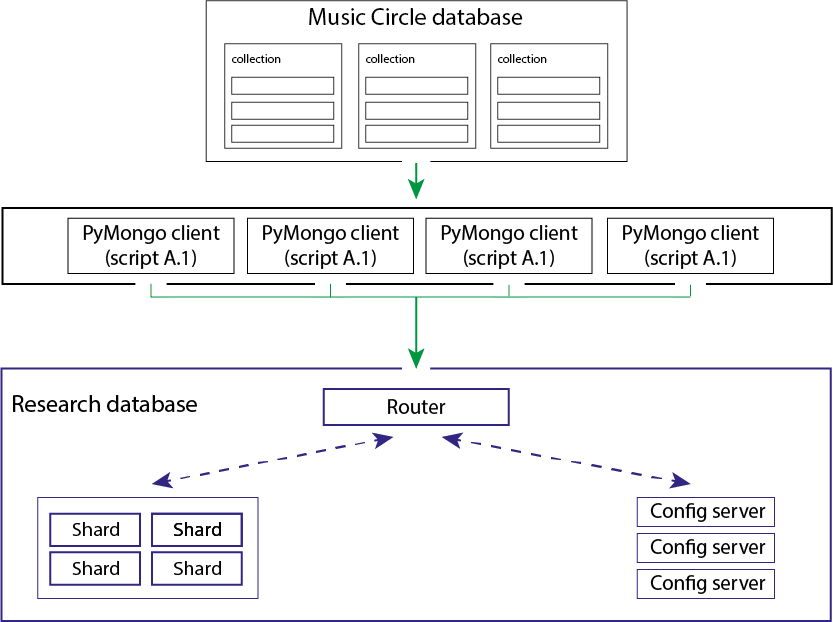
\includegraphics[width=0.6\textwidth]{./datapipe.png}
      \caption{Data flow between the Music Circle and Research database showing a Mongo sharded cluster}
      \label{figure:datapipeline}
\end{figure}

%\begin{table}[h]
%	\centering
%	\begin{tabular}{| l | l |}
%		\hline
%		 \textbf{Scripts} & \textbf{Description}\\ \hline
%		 \ref{importScript} & Inserts users, media, comments and replies to the Research database\\ \hline
%		 \ref{importShard1},  \ref{importShard2},  \ref{importShard3},  \ref{importShard4} & Insert the events logged into the Research database. They run in parallel.\\ \hline
%	\end{tabular}
%	\caption{Scripts to build the Research database}
%	\label{table:scriptsResearchDatabase}
%\end{table}

\begin{table}[h!]
	\centering
	\begin{tabularx}{\linewidth}{|X|X|X|}
		\hline
		 \textbf{Collection} & \textbf{Description} & \textbf{Number of items} \\ \hline
		 Actors & Music Circle users & 3715 \\ \hline
		 Sessions & Music Circle users sessions & 11350 \\ \hline
		 Media & Media items uploaded & 2897 \\ \hline
		 Final Grades & Final grades from students & 50300\\ \hline
		 Final Grades in Research database & Students in the Research database that have grades & 1852\\ \hline
		 Total activities & Total activities in Music Circle & 8326972 \\ \hline
		 Comment & Comments posted & 7370\\ \hline
		 Community tracks views & Number of community tracks views & 351541 \\ \hline
		 Owned tracks views & Number of views on owned tracks & 9975 \\ \hline
		 Comments views & Number of comment views & 30351 \\ \hline
		 Plays & Number of plays & 36936 \\ \hline
		 Replies & Replies posted & 978 \\ \hline
	\end{tabularx}
	\caption{Summary of the data in the Research database}
	\label{table:researchDatabase}
\end{table}

\section{High level data analysis}
\label{section:statisticsStudy}
\subsection{Aim}
The aim of this study was to generate high level statistics. It was an opportunity to test the Research database and make the necessary adjustments in order to make it robust. Additionally, it was an opportunity to familiarise myself with Python and its scientific tools.

\subsection{Methods}
The first step was to explore the Music Circle database by showing the activities per day. Script [\ref{initialPerDayPlots}] iterates through various collections in the Music Circle database and counts how many activities happened per day. Figure \ref{figure:activityLevel} show the plots generated. The spikes in the plots correspond to a surge in activity due to the approach of assessment dates.
\begin{figure}
        \centering
        \begin{subfigure}[b]{0.45\textwidth}
                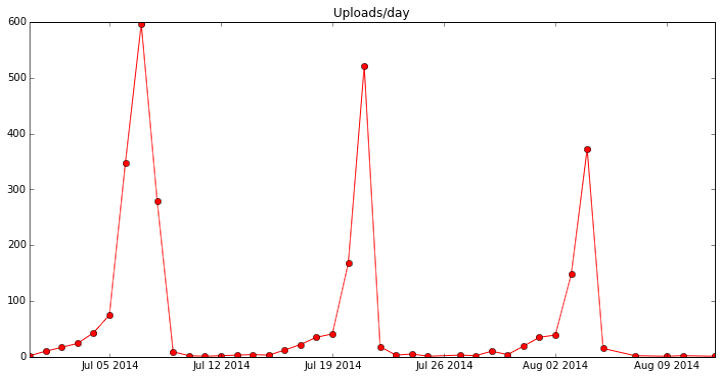
\includegraphics[width=\textwidth]{./uploadsPerDay.png}
                \caption{Uploads per day}
                \label{uploadsPerDay}
        \end{subfigure}%
        ~ %add desired spacing between images, e. g. ~, \quad, \qquad, \hfill etc.
          %(or a blank line to force the subfigure onto a new line)
        \begin{subfigure}[b]{0.45\textwidth}
                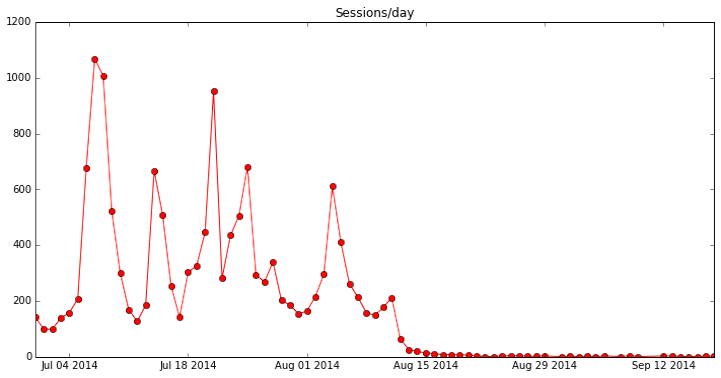
\includegraphics[width=\textwidth]{sessionsPerDay.png}
                \caption{Sessions per day}
                \label{sessionsPerDay}
        \end{subfigure}
        ~ %add desired spacing between images, e. g. ~, \quad, \qquad, \hfill etc.
          %(or a blank line to force the subfigure onto a new line)
        \begin{subfigure}[b]{0.45\textwidth}
                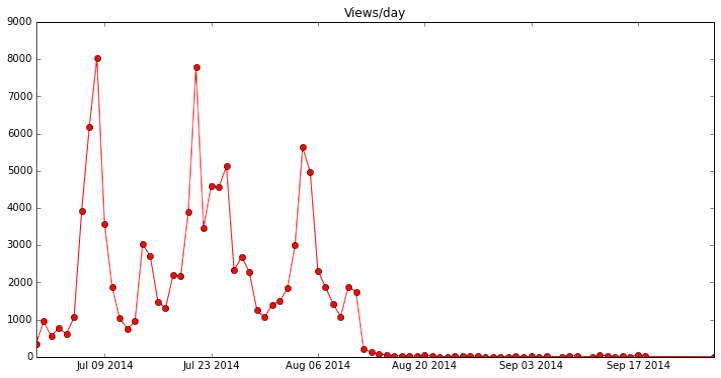
\includegraphics[width=\textwidth]{viewsPerDay.png}
                \caption{Views per day}
                \label{viewsPerDay}
        \end{subfigure}
        ~ %add desired spacing between images, e. g. ~, \quad, \qquad, \hfill etc.
          %(or a blank line to force the subfigure onto a new line)
        \begin{subfigure}[b]{0.45\textwidth}
                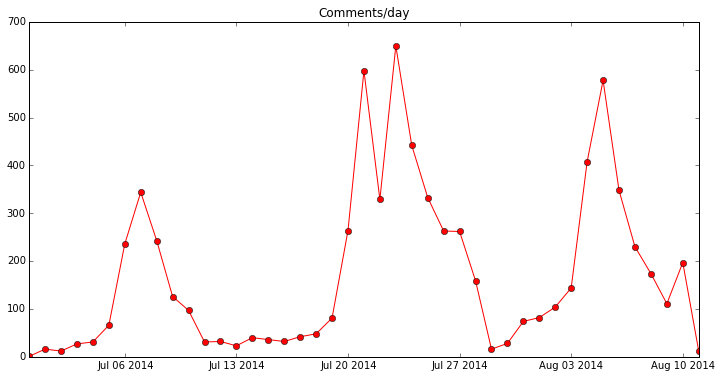
\includegraphics[width=\textwidth]{commentsPerDay.png}
                \caption{Comments per day}
                \label{commentsPerDay}
        \end{subfigure}
        ~ %add desired spacing between images, e. g. ~, \quad, \qquad, \hfill etc.
          %(or a blank line to force the subfigure onto a new line)
        \begin{subfigure}[b]{0.45\textwidth}
                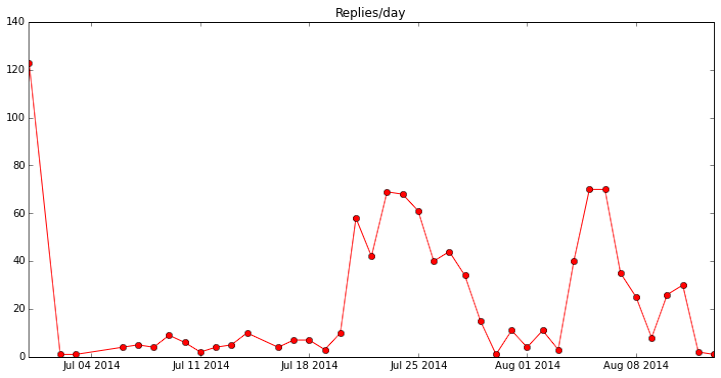
\includegraphics[width=\textwidth]{repliesPerDay.png}
                \caption{Replies per day}
                \label{repliesPerDay}
        \end{subfigure}
        \caption{Plots showing activity level over time}
        \label{figure:activityLevel}
\end{figure}
\\\\After these initial statistics, the data in the Research database was explored. A necessary step was to clean the data as much as possible. After trying to implement initial statistics I realised that some user events were logged more than once. Those duplicates had to be removed since they would interfere with the results. Script [\ref{removeDuplicates}] removes the duplicates in the activities array. For each user it iterates through the activities array, it finds the duplicates and it removes them from the database.\\\\ 
As said before, this study was an opportunity to explore the data. Particularly interesting were the extreme cases of very active or very inactive users. Therefore, a script [\ref{countActivitiesAndUploads}] that added some information into the Actors collection elements about the students' level of activity was implemented, specially since Mongo query modifiers can not operate array length queries.\\\\ 
After this data cleaning step it was time to link the Research database with the Coursera database that contains the ground truth (final grades of students). The process of linking the two databases consists in matching user ids in order to connect users in the Research database with final grades in the Coursera database. Figure \ref{figure:linkDatabases} shows the matching process. In the PraiseUser table in the Music Circle database there is a field called {\it courseraId} which in theory allows to link with the Coursera database that contains the final grades student achieved. Unfortunately, this is not the case and none of the {\it courseraIds} were present in the Coursera database. This was a major issue since without being able to link both databases this project could not be completed. The script that solves this issue is [\ref{dbLink}] and this is the approach considered: Each submission on Coursera contains a session id and a link to a particular item in Music Circle. The session id matches a row in the Coursera database. The link to Music Circle contains a media id at the end of it. Media items in the Music Circle contain the user id that owns them. This way there is a link between the Coursera database and the Music Circle database. The data was inserted in a new collection in the research database called ActorsGrade where each element contains the Music Circle user id, the grade achieved from the Coursera database and the total number of activities performed by the user.\\ 
Not all the users in the Coursera database could be matched to the Research database because some students either did not finish the course or did not upload media to Music Circle. A total of 1,852 students in the Research database have a final grade.
\clearpage
\begin{figure}[h!]
        \centering
   	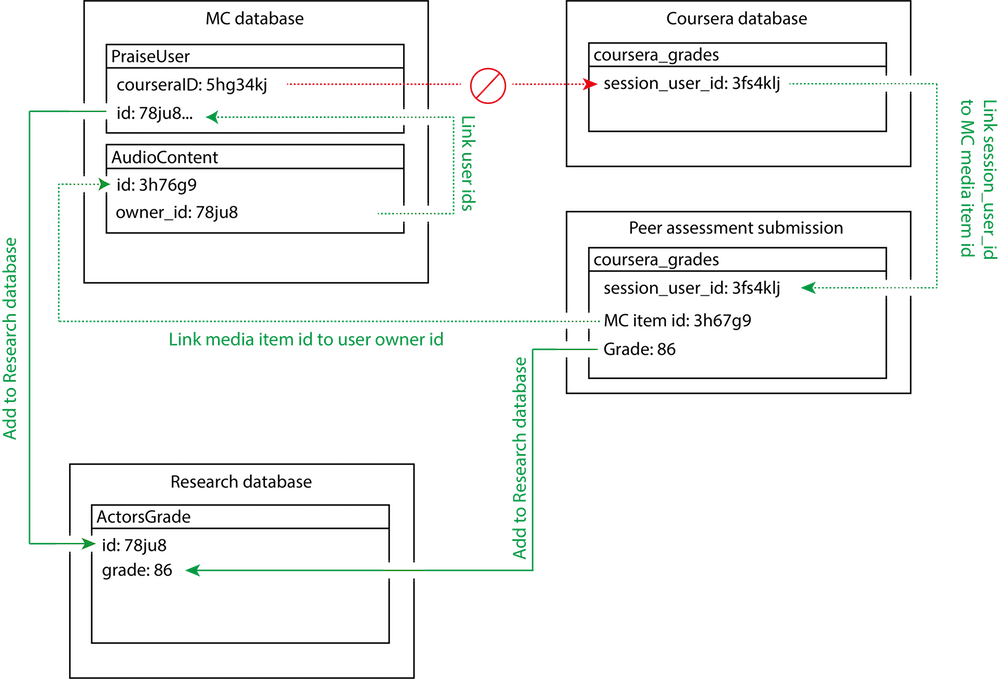
\includegraphics[width=0.8\textwidth]{./dbLink.png}
    	\caption{Linking Music Circle, Coursera and Research databases}
	\label{figure:linkDatabases}
\end{figure}
\noindent The final step was to generate plots comparing activity levels to final grades. Figure \ref{figure:activityCorrelationWithGrades} show the plots generated by script  [\ref{groundTruth}].
\begin{figure}
        \centering
        \begin{subfigure}[b]{0.4\textwidth}
                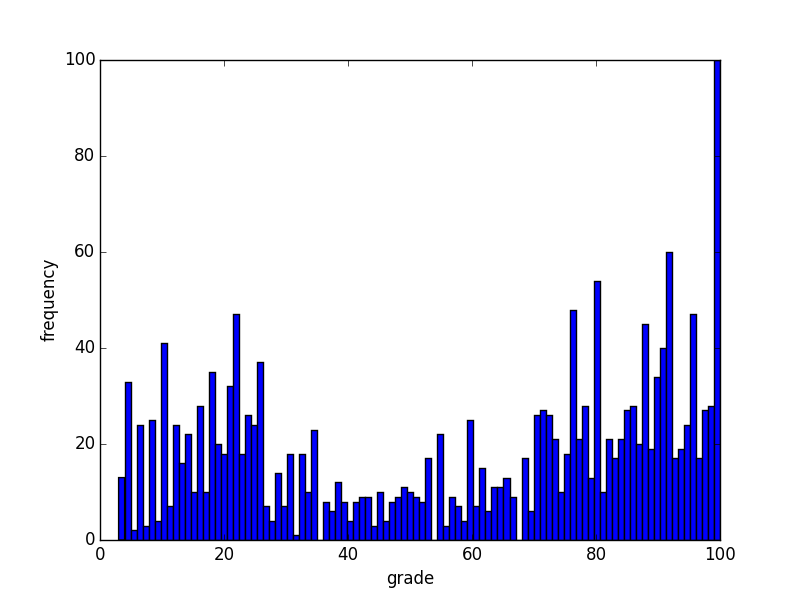
\includegraphics[width=\textwidth]{./pythonScripts/generalStatistics/distributionGrades.png}
                \caption{Distribution of grades}
                \label{distOfGrades}
        \end{subfigure}
        ~ %add desired spacing between images, e. g. ~, \quad, \qquad, \hfill etc.
          %(or a blank line to force the subfigure onto a new line)
         \begin{subfigure}[b]{0.4\textwidth}
                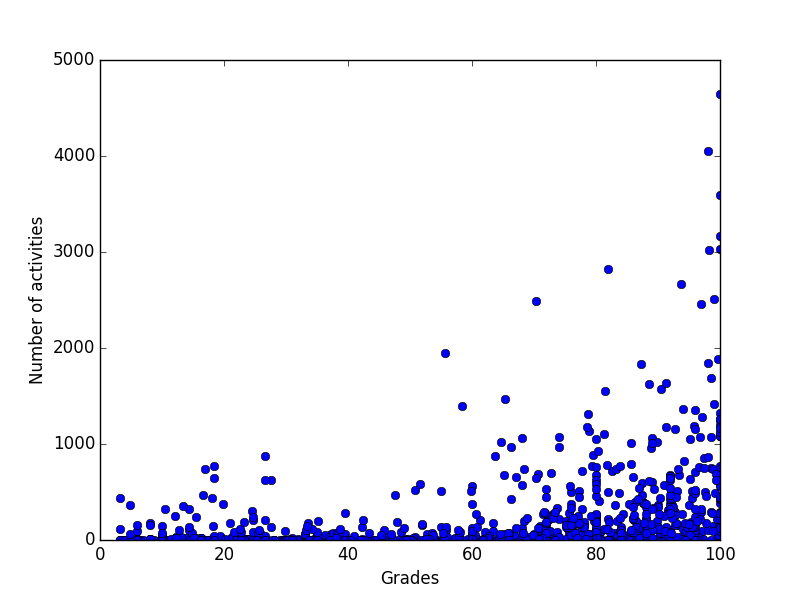
\includegraphics[width=\textwidth]{./pythonScripts/allActivities.png}
                \caption{Total activities vs grades}
                \label{actVSgrades}
        \end{subfigure}
        ~ %add desired spacing between images, e. g. ~, \quad, \qquad, \hfill etc.
          %(or a blank line to force the subfigure onto a new line)
        \begin{subfigure}[b]{0.4\textwidth}
                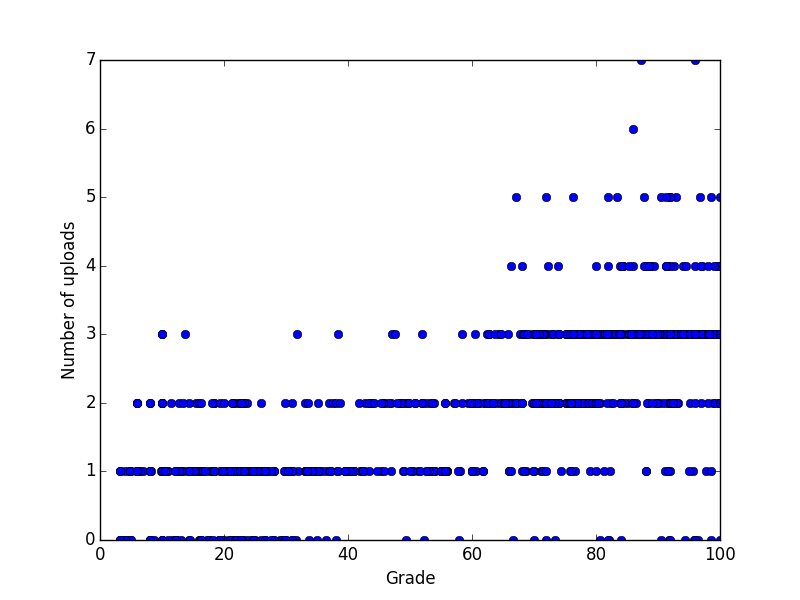
\includegraphics[width=\textwidth]{./pythonScripts/generalStatistics/uploads.png}
                \caption{Uploads vs grades}
                \label{Uploads}
        \end{subfigure}
        ~ %add desired spacing between images, e. g. ~, \quad, \qquad, \hfill etc.
          %(or a blank line to force the subfigure onto a new line)
        \begin{subfigure}[b]{0.4\textwidth}
                 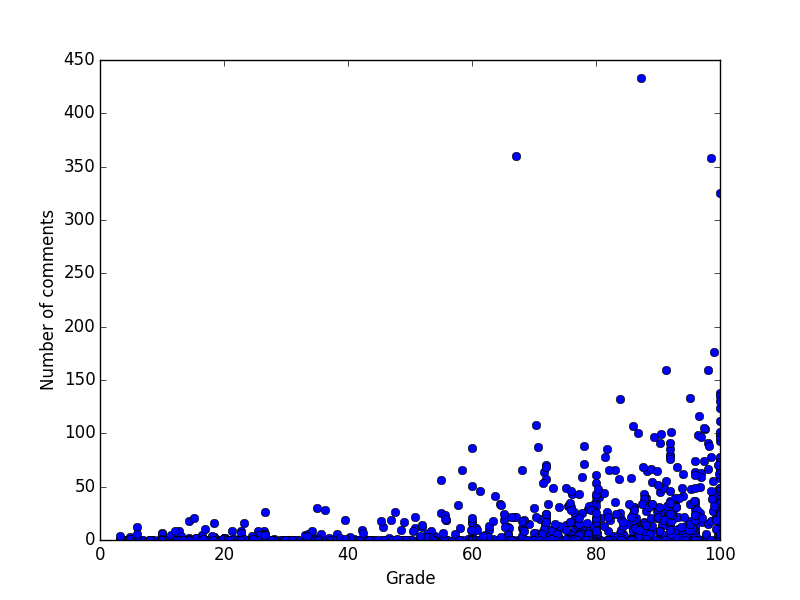
\includegraphics[width=\textwidth]{./pythonScripts/generalStatistics/comments.png}
                 \caption{Comment views vs grades}
                 \label{comments}
         \end{subfigure}
        ~ %add desired spacing between images, e. g. ~, \quad, \qquad, \hfill etc.
          %(or a blank line to force the subfigure onto a new line)
        \begin{subfigure}[b]{0.4\textwidth}
                 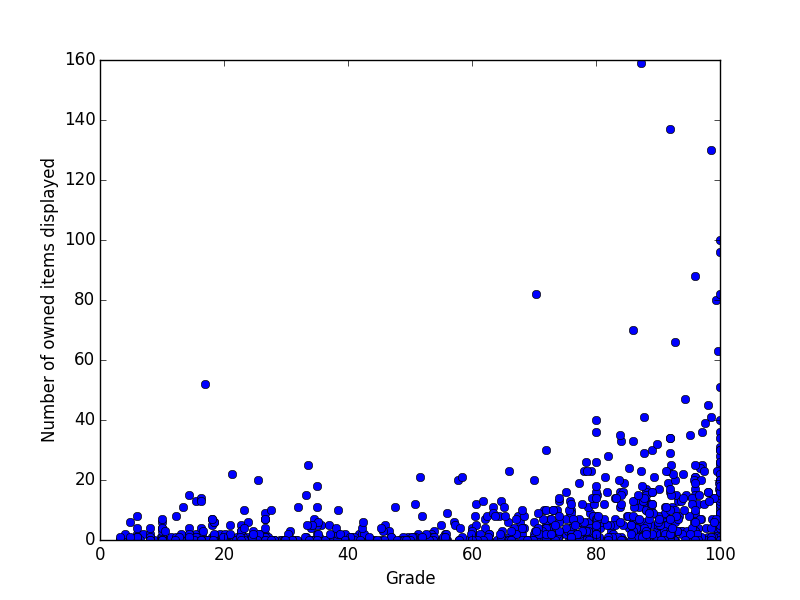
\includegraphics[width=\textwidth]{./pythonScripts/generalStatistics/mytracks.png}
                 \caption{Owned track views vs grades}
                 \label{mytracks}
         \end{subfigure}
         ~ %add desired spacing between images, e. g. ~, \quad, \qquad, \hfill etc.
           %(or a blank line to force the subfigure onto a new line)
	\begin{subfigure}[b]{0.4\textwidth}
                 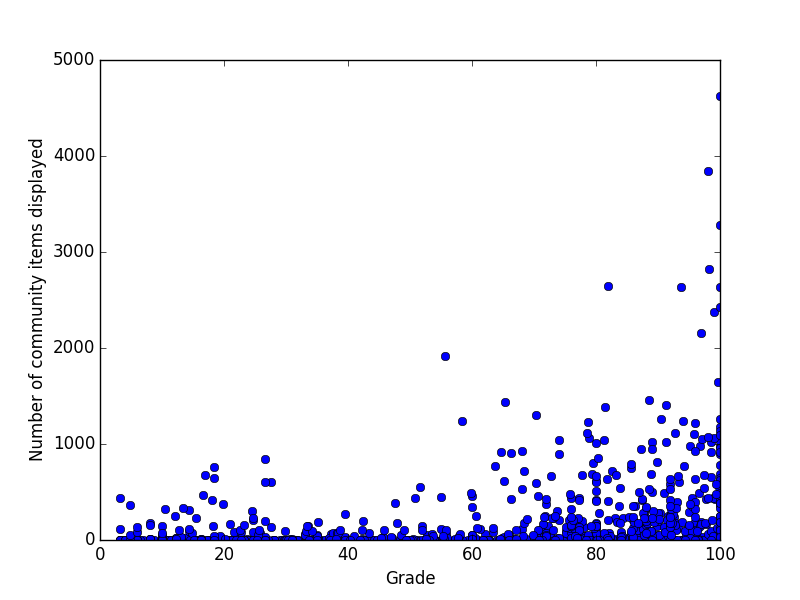
\includegraphics[width=\textwidth]{./pythonScripts/generalStatistics/community.png}
                 \caption{Community track views vs grades}
                 \label{communityTracks}
         \end{subfigure}
         ~ %add desired spacing between images, e. g. ~, \quad, \qquad, \hfill etc.
           %(or a blank line to force the subfigure onto a new line)
	\begin{subfigure}[b]{0.4\textwidth}
                 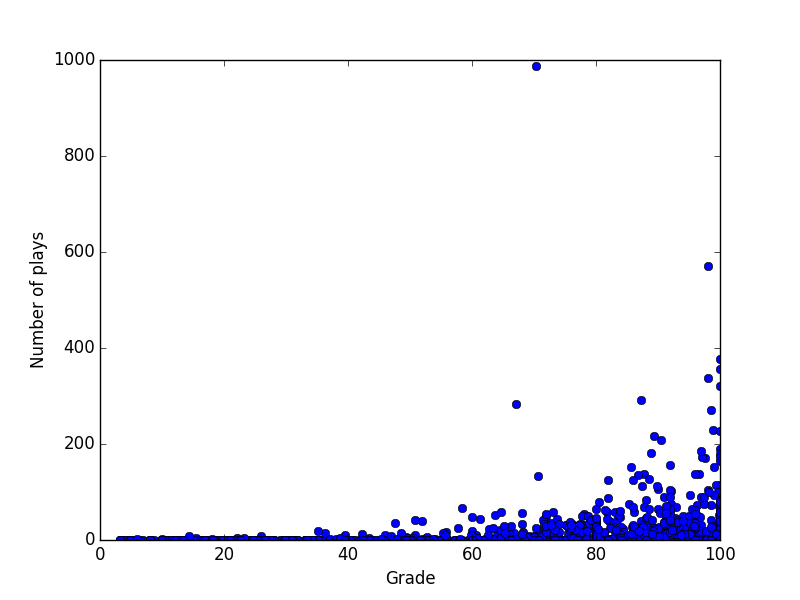
\includegraphics[width=\textwidth]{./pythonScripts/generalStatistics/plays.png}
                 \caption{Number of plays vs grades}
                 \label{plays}
         \end{subfigure}
         ~ %add desired spacing between images, e. g. ~, \quad, \qquad, \hfill etc.
           %(or a blank line to force the subfigure onto a new line)
        \begin{subfigure}[b]{0.4\textwidth}
                 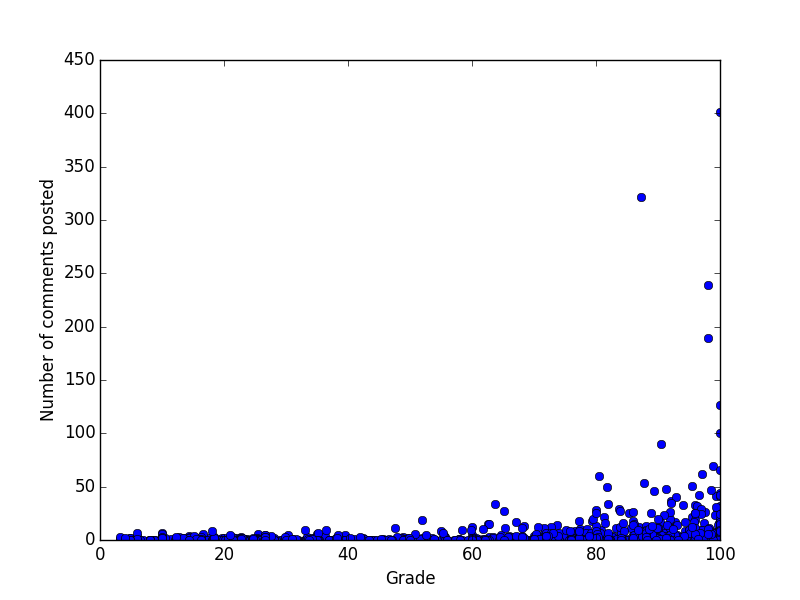
\includegraphics[width=\textwidth]{./commentsPostedVsGrades.png}
                 \caption{Comments posted vs grades}
                 \label{commentsPosted}
         \end{subfigure}
         ~ %add desired spacing between images, e. g. ~, \quad, \qquad, \hfill etc.
           %(or a blank line to force the subfigure onto a new line)
        \caption{Correlation between activity levels and grades}
        \label{figure:activityCorrelationWithGrades}
\end{figure}
\newpage
% Talk about regression?
\subsection{Conclusion}
This study had different aims: To complete the research database, to explore the data and to present statistics that would hopefully offer clues on how to analyse the data. From the plots it is obvious that there is not a predominant correlation between activities and grades for any of the measures. The analytical results from the linear regressions support this by showing a coefficient of correlation close to 0. The results are presented in Table \ref{table:initialStudyResults}. Trying to fit non linear functions might improve the results. The data does not show any signs of a defined probability distribution, making it difficult to decide what the next steps are. 
\begin{table}[h]
	\centering
	\begin{tabular}{| l | l |}
		\hline
		 \textbf{Activity} & \textbf{$r^2$} \\ \hline
		 Uploads & 0.5067 \\ \hline
		 Comments views & 0.1576 \\ \hline
		 Owned tracks views & 0.1211 \\ \hline
		 Community tracks views & 0.1034 \\ \hline
		 Plays & 0.1154 \\ \hline
		 Comments posted & 0.1364 \\ \hline
	\end{tabular}
	\caption{Results of linear regressions on the different statistics}
	\label{table:initialStudyResults}
\end{table}
\newpage

\section{Exploratory data analysis}
\label{section:exploratoryDataAnalysis}
\subsection{Aim}
This section presents three studies that explore user behaviour using indictors of feedback activity. Section \ref{subsection:differenceActivityFeedback} presents a method to construct feature vectors that allow for user differentiation. Section \ref{subsection:kNearestNeighbourStudy} presents a method to classify students based on their feedback activity in Music Circle. Section \ref{subsection:kMeansStudy} contains a higher resolution analysis of the user activity after feedback. Finally, Section \ref{conclusion} contains a summary of the results of the three studies.
\subsection{Difference on feedback activity between users}
The method presented in Section \ref{section:statisticsStudy} failed at finding correlations between student feedback activity and student performance. This study proposes to consider the relations between the different feedback activities in order to find similarities between users. In order to do this, the first step is to construct a data structure that allows a multidimensional comparison of students considering all the different feedback activities. This is achieved by building a feature vector that contains feedback activity information. Each student has associated a feature vector that contains information about the feedback activities of that particular student. Once built, these vectors allow us to use Euclidian distance to make comparisons between students.\\\\
For this study, the feature vector had this form:
\begin{equation}
v_n=[u,c,m,g,p]
\label{featureVector1}
\end{equation}
Where:
\begin{itemize}
	\item $n$ = user
	\item $u$ = total number of uploads for user $n$
	\item $c$ = total number of comment views for user $n$
	\item $m$ = total number of media views for user $n$
	\item $g$ = total number of community media views for user $n$
	\item $p$ = total number of plays for user $n$
\end{itemize}
The Research database contains the data used to calculate the different components of the feature vectors. Each element in the Actors collection contains information about the activity of a particular student using Music Circle. We consider feedback activities the ones that present information to the students, in Music Circle those activities are triggered by mouse clicks events. Each component of the feature vector contains the total number of clicks on different elements on the Music Circle interface. For example, the $p$ component is calculated counting how many times a user clicked on the play button. The period of time considered is the total length of the case study. The use of cumulative measures of events is suggested by Maia \cite{Maia2008}. Moreover, this feature vector is intuitive and easy to calculate.\\\\
Table \ref{table:featureVectorsInitial} contains examples of feature vectors calculated.
\begin{table}[h]
	\centering
	\begin{tabular}{| l | l |}
		\hline
		 \textbf{Users} & \textbf{Feature Vectors} \\ \hline
		 A & [2, 25, 30, 89, 23] \\ \hline
		 B & [0, 7, 0, 737, 7] \\ \hline
		 C & [1, 0, 1, 102, 19] \\ \hline
		 D & [0, 77, 7, 0, 59] \\ \hline
	\end{tabular}
	\caption{Examples of feature vectors}
	\label{table:featureVectorsInitial}
\end{table}
\\Once the feature vectors were built, they were plotted in order to visually inspect them. Script [\ref{featureVectorsHistograms}] calculates the feature vectors, generates histograms for each of the feature vectors and saves them as a .png file. Only users with more than 100 activities logged are considered which produced 664 plots. Once the .png images were generated, a video of them was created using FFMPEG \cite{ffmpeg}. The video was made in order to be able to watch all the images in a short period of time, the hope was to visually detect similarities in the data which would indicate similar user behaviour. The video can be found here: \url{http://youtu.be/cnBnJAWI9ro}. Unfortunately, no obvious patterns were detected. Figure \ref{figure:histogramForDifferentUsers} shows several histograms corresponding to different users.
\begin{figure}[!htb]
        \centering
        \begin{subfigure}[b]{0.45\textwidth}
                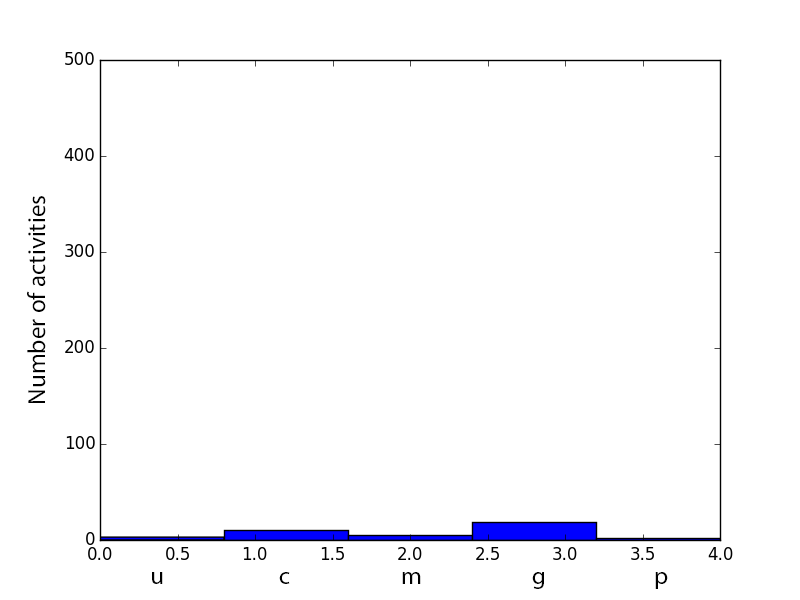
\includegraphics[width=\textwidth]{./hist1.png}
                \caption{Histogram of the feature vector}
                \label{hist1}
        \end{subfigure}
        ~ %add desired spacing between images, e. g. ~, \quad, \qquad, \hfill etc.
          %(or a blank line to force the subfigure onto a new line)
        \begin{subfigure}[b]{0.45\textwidth}
                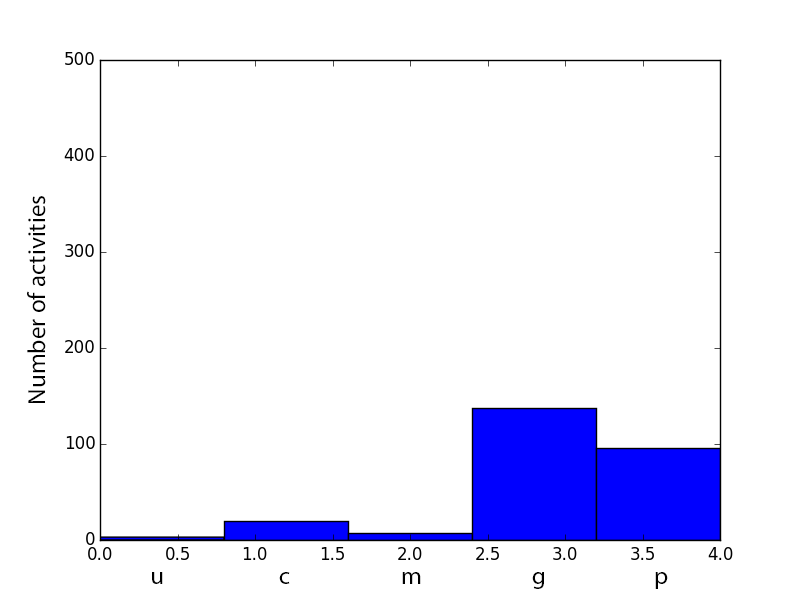
\includegraphics[width=\textwidth]{./hist2.png}
                \caption{Histogram of the feature vector}
                \label{hist2}
        \end{subfigure}
        ~ %add desired spacing between images, e. g. ~, \quad, \qquad, \hfill etc.
          %(or a blank line to force the subfigure onto a new line)
        \begin{subfigure}[b]{0.45\textwidth}
                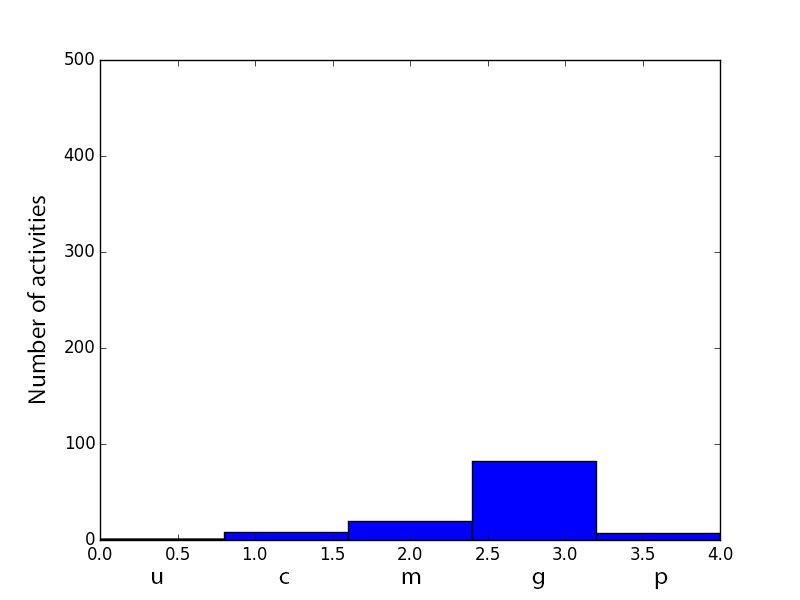
\includegraphics[width=\textwidth]{./hist3.png}
                \caption{Histogram of the feature vector}
                \label{hist3}
        \end{subfigure}
        ~ %add desired spacing between images, e. g. ~, \quad, \qquad, \hfill etc.
          %(or a blank line to force the subfigure onto a new line)
        \begin{subfigure}[b]{0.45\textwidth}
                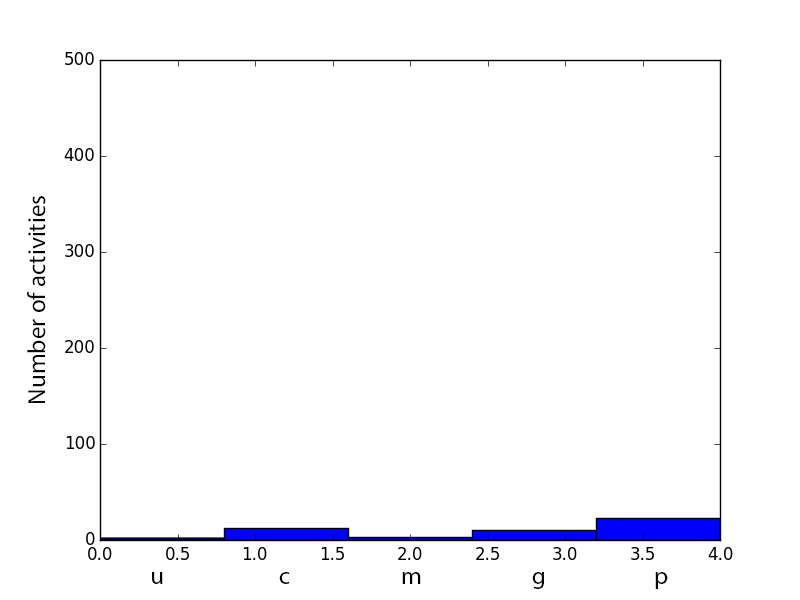
\includegraphics[width=\textwidth]{./hist4.png}
                \caption{Histogram of the feature vector}
                \label{hist4}
        \end{subfigure}
        ~ %add desired spacing between images, e. g. ~, \quad, \qquad, \hfill etc.
          %(or a blank line to force the subfigure onto a new line)
        \begin{subfigure}[b]{0.45\textwidth}
                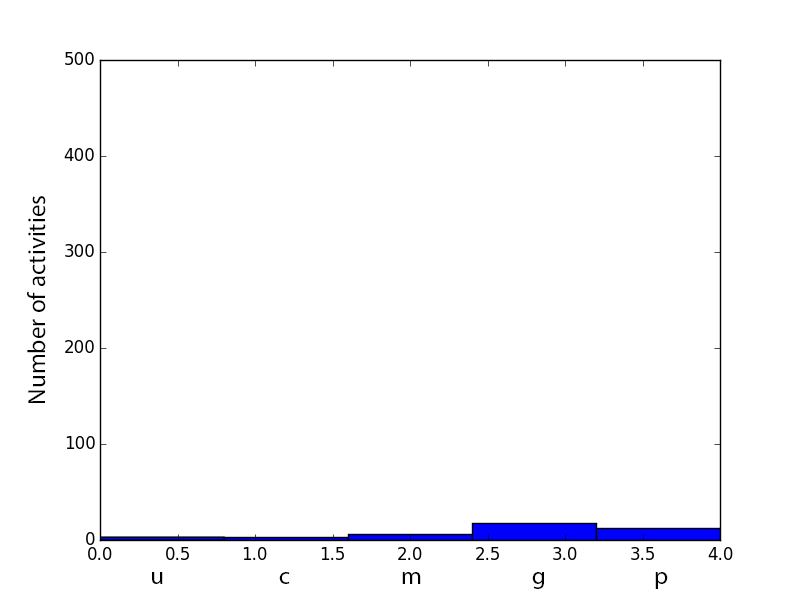
\includegraphics[width=\textwidth]{./hist5.png}
                \caption{Histogram of the feature vector}
                \label{hist5}
        \end{subfigure}
        ~ %add desired spacing between images, e. g. ~, \quad, \qquad, \hfill etc.
          %(or a blank line to force the subfigure onto a new line)
        \begin{subfigure}[b]{0.45\textwidth}
                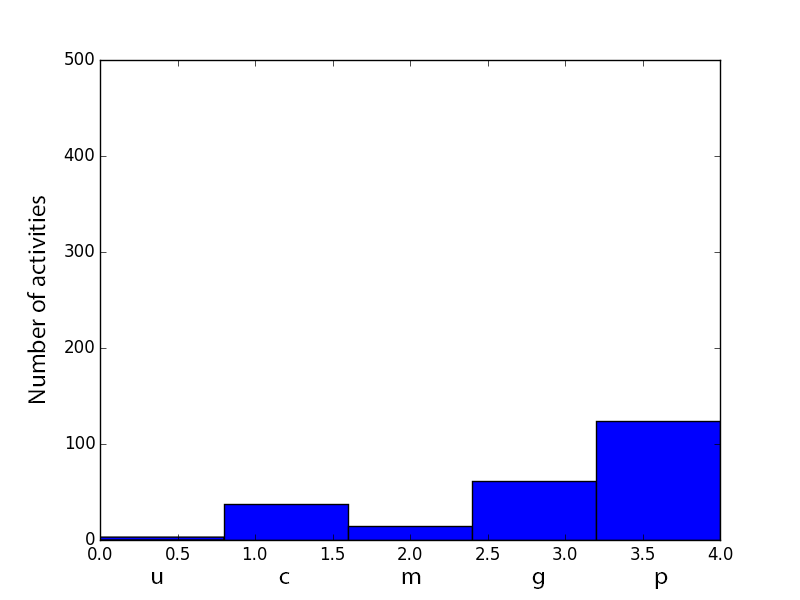
\includegraphics[width=\textwidth]{./hist6.png}
                \caption{Histogram of the feature vector}
                \label{hist6}
        \end{subfigure}
	\caption{Feature vector histograms for different users}
	\label{figure:histogramForDifferentUsers}
\end{figure}
\clearpage
\noindent The video generated provides a high level overview of the feature vectors. For example, it shows that viewing group media items and playing media items are popular activities between all users.\\ Something that was unknown at this stage was whether the feature vectors were suited to differentiate users. The video shows how the different feature vectors change, proving that in general different users had different vectors. However, it had to be proven that these differences were enough to differentiate between users.\\\\ %The intention of making a video was not to find an analytical result but to provide with a quick visual method to inspect the feature vectors hoping that it would provide hints on how to proceed with the analysis in trying to find a method to find similar users.\\\\
In order to provide with analytical data about the differences between users a difference matrix was calculated. To do so, the Euclidian distance from each feature vector to all the others is calculated and stored in a matrix. Each row of the matrix contain the distances between a unique feature vector and all the others. %The feature vectors are calculated as described by Equation \ref{featureVector1}.
\\After a close inspection of the data used to construct the feature vectors it was discovered that some of the events logged were very close in time with less than 50ms between them. Those events are the result of 'double clicks' or other artefacts, they do not add any valuable information and it was decided to remove them from the dataset. Additionally, the feature vectors were normalised so that their length would always be 1. This removes dependancies in the number of events performed by the students and adds information about the relationships (and proportions) of each activity with respect to the other activities. Script [\ref{featureVectorsNoSessions}] calculates the feature vectors and stores them into a JSON file. There is one feature vector per user. Script [\ref{distanceMatrix}] calculates the Euclidian distance from each feature vector to all the others and it stores it in a matrix. Figure \ref{figure:heatplot} shows a heat map of the distance matrix, it is generated by script [\ref{heatPlot}].\\\\
In the heat map, clear areas indicate similarity (small distances) whereas dark areas indicate dissimilarity (large distances). It is a proof that the feature vectors calculated can distinguish between users.

\begin{figure}[h!]
        \centering
        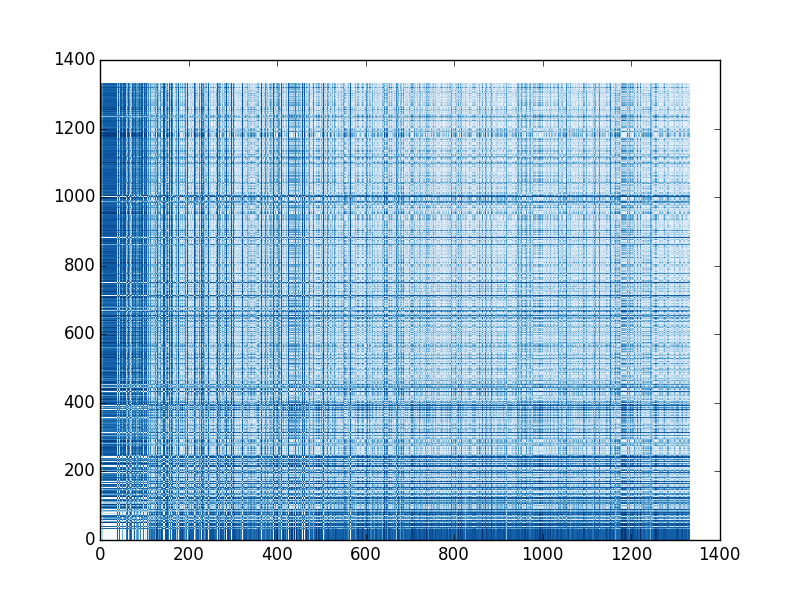
\includegraphics[width=0.6\textwidth]{./pythonScripts/heatmap2.png}
        \caption{Heat map of the distance matrix}
	\label{figure:heatplot}
\end{figure}
\label{subsection:differenceActivityFeedback}

\subsection{K-Nearest neighbour classification}
The previous study shows how the feature vectors can differentiate between users. This section proposes a method to classify students into performance categories based on the feedback activity. The method chosen for the classification is a $k$-nearest neighbour algorithm.\\\\
Given a dataset $D$ and a point $p \in D$, the $k$-Nearest Neighbour (KNN) algorithm finds the $k$ closest points to $p$ where $k \in D$. It is a well known data mining method that can be used for classification and regression.\\ 
For classification, the algorithm consists in associating a class $C$ to each of the points in $D$. It calculates the distance from $p$ to all the points in $D$. The calculated distances are sorted in a decreasing order and the smallest $k$ are chosen. Each of the distances is associated with a point $p'$ and a class $C$, the majority of classes is chosen as the class of $p$.\\ The KNN implementation is provided by {\it scikit-learn} \cite{scikit} which is a machine learning library for Python which contains tools for data mining and data analysis. It is built on Numpy, SciPy and matplotlib, making it fully compatible with Python scientific programming tools.\\\\
As in the previous study. Feature vectors that describe feedback activity need to be built. Each element in the Actors collection contains information about the activity of a particular student using Music Circle. We consider feedback activities the ones that present information to the students, in Music Circle those activities are triggered by mouse clicks events. Each component of the feature vector contains the total number of clicks on different elements on the Music Circle interface. For example, the $u$ component is calculated counting the total number of uploads of a user. The period of time considered is the total length of the case study. The feature vectors constructed are very similar to the ones used in Section \ref{subsection:differenceActivityFeedback} but add an extra component that measures the total number of comments posted. For this study, the feature vector had this form:
\begin{equation}
v_n=[u,c,m,g,p,cm]
\label{featureVectorKNN}
\end{equation}
Where:
\begin{itemize}
	\item $n$ = user
	\item $u$ = total number of uploads for user $n$
	\item $c$ = total number of comment views for user $n$
	\item $m$ = total number of media views for user $n$
	\item $g$ = total number of community media views for user $n$
	\item $p$ = total number of plays for user $n$
	\item $cm$ = total number of comments posted for user $n$
\end{itemize}
The different components are calculated considering the full length of the case study. Table \ref{table:featureVectorsKNN} contains examples of feature vectors calculated.\\\\
\begin{table}[h]
	\centering
	\begin{tabular}{| l | l |}
		\hline
		 \textbf{Users} & \textbf{Feature Vectors} \\ \hline
		 A & [0.0435, 0.1159, 0.1014, 0.1884, 0.3043, 0.2464] \\ \hline
		 B & [0.0857, 0.1429, 0.3714, 0.2571, 0.1143, 0.0286] \\ \hline
		 C & [0.0385, 0.1154, 0.2115, 0.5384, 0.0000, 0.0962] \\ \hline
		 D & [0.0789, 0.0000, 0.47367, 0.2632, 0.1579, 0.0263] \\ \hline
	\end{tabular}
	\caption{Examples of feature vectors}
	\label{table:featureVectorsKNN}
\end{table}
\\Script \ref{knn} trains a KNN algorithm to classify students. The first step is to generate the classes and assign them to the students. Three classes are considered:
\begin{itemize}
	\item Students that achieved $<$ 50 on their final grade
	\item Students that achieved between 50 and 70 on their final grade
	\item Students that achieved $>=$ 70 on their final grade
\end{itemize}
\vspace{5mm}
In order to use KKN the value of $k$ needs to be specified. In order to choose the best value for $k$ one must try different $k$ and choose the one that provides better results. Therefore, one needs a method to validate the performance of the algorithm. The method chosen to measure the performance of the classification is commonly referred as cross-validation.\\\\
In order to cross-validate the KKN algorithm, the dataset is split into a training and test dataset in a 90/10 ratio. The training dataset is used to train the KKN algorithm whereas the test dataset is used to test its performance. %As seen in section X it was not possible to obtain the final grade of all the users. Moreover, both datasets contain a randomised selection of the original dataset, therefore, each time the algorithm is run different results are expected.\\\\
The performance metric used to determine the optimal $k$ is the accuracy of the classification. As seen in section \ref{section:statisticsStudy}, it was not possible to obtain the final grade of all the users. Moreover, both datasets contain a randomised selection of the original dataset, therefore, each time the algorithm is run different results on the accuracy of the algorithm are expected.\\\\
The algorithm was run for a range of $k$ varying from $k$=2 to $k$=80, for each $k$ the algorithm was run 100 times and the accuracy of the classification was calculated. Figure \ref{figure:knnFigure} presents the results of the accuracy versus $k$, each point consists in the mean accuracy value, the error bars consist in the range of accuracies calculated for a particular $k$.
\begin{figure}
        \centering
        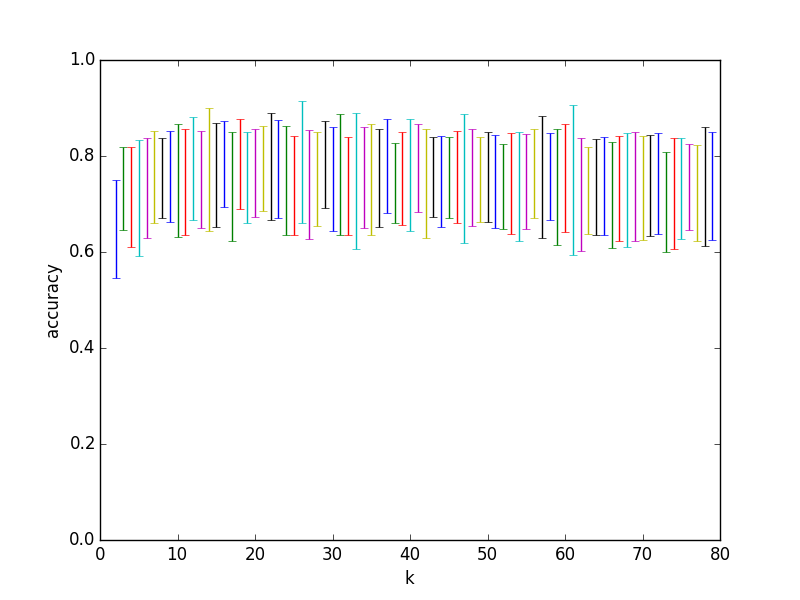
\includegraphics[width=0.6\textwidth]{./pythonScripts/kNeighbours.png}
        \caption{Accuracy of the classification using KNN with cross-validation}
	\label{figure:knnFigure}
\end{figure}
The greatest accuracy is obtained for $k$=24 with a value of $a$=0.7980. Once the optimal $k$ was determined other performance metrics were calculated. Accuracy measures the proportion of corrected classified instances. Precision measures the fraction of instances that are relevant. Recall measures the fraction of relevant instances that are retrieved. Finally, F1 is the harmonic mean between the precision and the recall. Table \ref{table:performanceMetrics} shows all the performance metrics calculated.
\begin{table}[h!]
	\centering
	\begin{tabular}{| l | l |}
		\hline
		 \textbf{Metric} & \textbf{Value} \\ \hline
		 Accuracy & 0.7980\\ \hline
		 Precision & 0.7300 \\ \hline
		 Recall & 0.8000 \\ \hline
		 F1 & 0.7600 \\ \hline
	\end{tabular}
	\caption{Performance metrics for the KNN classification}
	\label{table:performanceMetrics}
\end{table}
\label{subsection:kNearestNeighbourStudy}
\clearpage
\subsection{In-depth analysis of feedback activity}
The aim of this study was to analyse the feedback activity with a higher resolution with respect to the studies described in sections \ref{subsection:differenceActivityFeedback} and \ref{subsection:kNearestNeighbourStudy}.\\ 
An interesting question is to consider user activity just after feedback. In order to do so, a new method to construct feature vectors is needed. This new method will have to solve the difficult question of determining for how long a particular feedback action has effect.\\\\
In this study it is assumed that the effects of feedback last through a whole user session. A session is the period of time between the login of the user and the logout on Music Circle. Script [\ref{makeSessions}] imports the sessions for each user. It finds all the actors in the research database that have activities or uploads, it then iterates through the found actors and finds all the session in the Music Circle database for each user. Once the sessions are retrieved, the right actor in the research database is found and a new field called {\it sessions} is inserted. Figure \ref{figure:sessions2} illustrates this process.
\begin{figure}[h!]
  \centering
    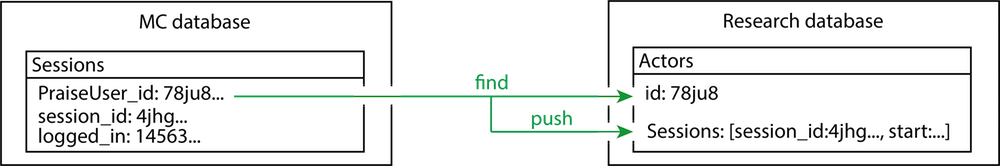
\includegraphics[width=0.6\textwidth]{./sessions.png}
      \caption{Import sessions into the research database}
      \label{figure:sessions2}
\end{figure}
\\The process of building the feature vectors is similar to the one followed on sections \ref{subsection:differenceActivityFeedback} and \ref{subsection:kNearestNeighbourStudy}. The difference is that on this study each feature vector describes the user behaviour on one session as opposed as the whole case study. Therefore, each user has a set of feature vectors (one per session) instead of just one that considers the whole MOOC.\\\\
For this study, the feature vector had this form:
\begin{equation}
v_n=[u,c,m,g,p]
\label{featureVector3}
\end{equation}
Where:
\begin{itemize}
	\item $n$ = user
	\item $u$ = total number of uploads for user $n$
	\item $c$ = total number of comment views for user $n$
	\item $m$ = total number of media views for user $n$
	\item $g$ = total number of community media views for user $n$
	\item $p$ = total number of plays for user $n$
\end{itemize}
The different components are calculated considering the full length of a session. Table \ref{table:featureVectorsKMeanss} contains examples of feature vectors calculated.\\\\
\begin{table}[h]
	\centering
	\begin{tabular}{| l | l |}
		\hline
		 \textbf{Users} & \textbf{Set of feature vectors} \\ \hline
		 A & [0, 5, 0, 958, 5],[1, 1, 0, 0, 4]... \\ \hline
		 B & [0, 0, 0, 0, 0],[0, 21, 4, 468, 14]... \\ \hline
		 C & [0, 0, 1, 0, 0], [0, 0, 0, 8, 0]... \\ \hline
		 D & [0, 82, 1, 530, 23], [0, 25, 1, 123, 16]...\\ \hline
	\end{tabular}
	\caption{Examples of feature vectors}
	\label{table:featureVectorsKMeanss}
\end{table}

\noindent Script [\ref{featureVectorsToJson}] builds the feature vectors. The first step is to make a list of objects that contain the start and the end date of the sessions for each user. Then the list of activities is iterated making chunks of activities that happened in a particular session. These activities are stored in a matrix, each row contains a list of activities that happened during a particular session. The feature vectors are built by iterating the matrix and counting how many uploads, plays, clicks on owned media items, clicks on community media items and clicks on comments are per session. These values are put in a 5 dimensional vector. Therefore, for each session there is one feature vector. This process is repeated for all users and all the feature vectors are written in a Json file.\\\\
As in sections \ref{subsection:differenceActivityFeedback} and \ref{subsection:kNearestNeighbourStudy}, the feature vectors calculated need to be validated in order to prove that they can differentiate between users. The validation method considers the fact that there is a set of feature vectors for each user and assumes that each of those sets can characterise a particular user. These different sets of feature vectors form the ground truth, one can think of each set as a cluster  that describe a particular student behaviour. If the feature vectors describe users appropriately, taking all the feature vectors corresponding to all users and applying a $k$-clustering algorithm where $k$ is equal to the number of users should produce a similar clustering as the ground truth. The clustering generated can be compared to the ground truth in order to measure the quality of the clustering.\\\\
The clustering algorithm used on this study is $k$-means, it forms part of a wider group of methods called partition methods which are defined as follows: ``Given D, a data set of n objects, and k, the number of clusters to form, a partitioning algorithm organises the objects into k partitions ($k < n$), where each partition represents a cluster. The clusters are formed to optimise an objective partitioning criterion, such as a dissimilarity function based on distance, so that the objects within a cluster are similar, whereas the objects of different clusters are dissimilar in terms of the data set attributes'' \cite{Han:2005:DMC:1076797}.\\\\
The $k$-means algorithm takes $k$ as a parameter and partitions the data into $k$ clusters that have high intracluster similarity and low intercluster similarity. The cluster similarity is measured considering the mean of the elements in a cluster. Below there is a description on how the algorithm works:
\begin{itemize}
	\item Select $k$ random elements in the data that will be the initial cluster centres
	\item Each of the elements in the data is assigned to the centre cluster it is most similar according to a distance metrics (usually euclidian distance)
	\item The previous two steps iterate until a certain stoping criteria is fulfilled
\end{itemize}
The stopping criteria is usually determined by the square-error defined as follows $$E=\sum\limits_{i=1}^k\sum\limits_{p\in C}|p-m|^2$$
Script \ref{clustering} is responsible for the clustering of the feature vectors. The clustering algorithm is provided by {\it scikit-learn} \cite{scikit}. A $k$-means clustering with $k$ equal to the number of users is performed on all the feature vectors. Figure \ref{figure:clusteringGenerated} shows the result of the clustering generated whereas Figure \ref{figure:clusteringGroundTruth} shows the ground truth clustering. From a simple observation it is obvious that the two clusterings are different. However, in order to prove how different they are, similarity metrics are needed.
\begin{figure}[h!]
  \centering
    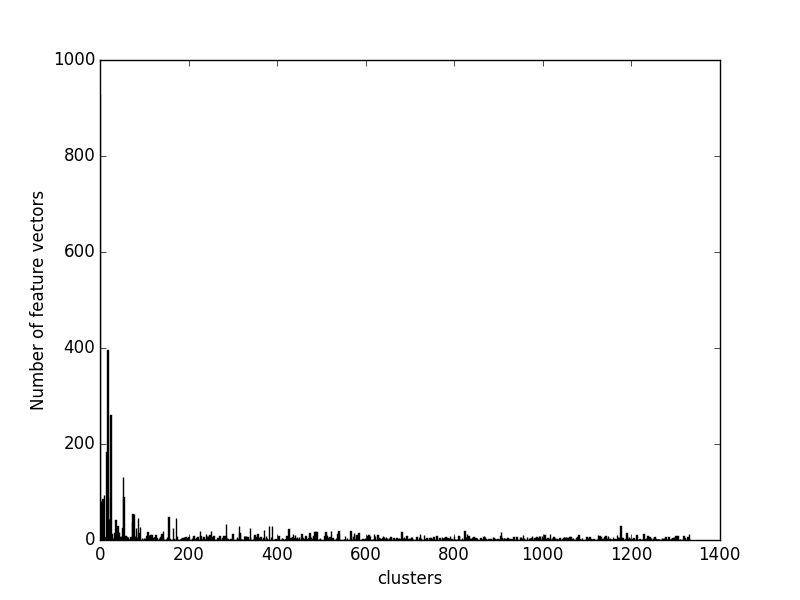
\includegraphics[width=0.6\textwidth]{./pythonScripts/histClusterGenerated.png}
      \caption{Clustering generated showing number of feature vectors per cluster. Each cluster represents a particular user.}
      \label{figure:clusteringGenerated}
\end{figure}
\begin{figure}[h!]
  \centering
    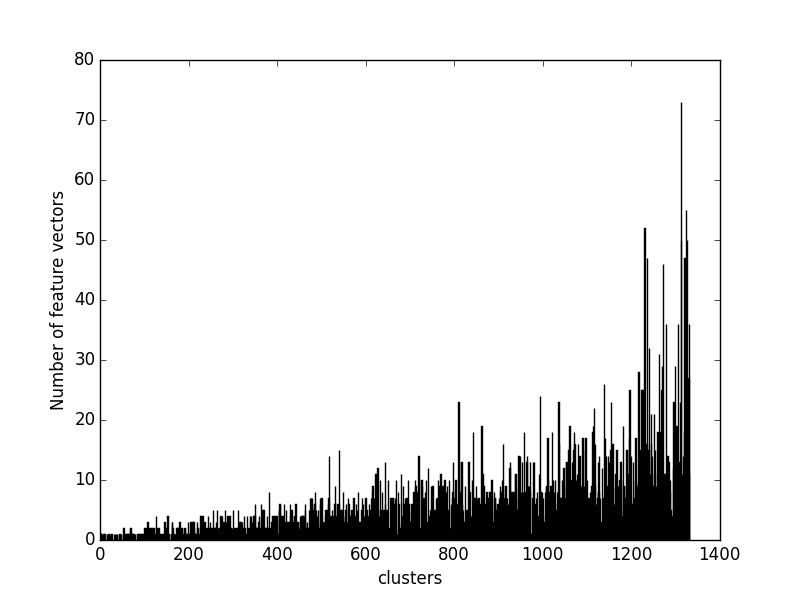
\includegraphics[width=0.6\textwidth]{./pythonScripts/histGroundTruth.png}
      \caption{Ground truth clustering. Data structure generated when calculating the feature vectors. Each user contains a set of feature vectors (cluster) that represent their behaviour.}
      \label{figure:clusteringGroundTruth}
\end{figure}
\newpage
\noindent The next step was to compare the ground truth clustering with the generated clustering. Script \ref{clusteringComparison} performed the clustering comparison by using different metrics. The adjusted random index computes a similarity measure between two clusterings by considering all pairs of samples and counting pairs that are assigned in the same or different clusters in the predicted and true clusterings \cite{scikit}. An adjusted random index with value 0 indicates that there is no difference between the calculated clustering and a random assignment whereas a value of 1 indicates perfect clustering.\\
The Mutual Information is a function that measures the agreement of the two assignments, ignoring permutations. Two different normalised versions of this measure are available, Normalised Mutual Information(NMI) and Adjusted Mutual Information(AMI). NMI is often used in the literature while AMI was proposed more recently and is normalised against chance. Values close to 0 indicate a random assignment whereas values close to 1 indicate equal clusters.\\
Homogeneity measures that each cluster contains members of a single class whereas completeness measures that all members of a single class are assigned to the same cluster. Additionally, the v-measure is the harmonic mean between homogeneity and completeness. Applying this measures to the ground truth and calculated clustering produces the results summarised in Table \ref{table:kMeansMetrics}.
\newpage
\begin{table}[h]
	\centering
	\begin{tabular}{| l | l |}
		\hline
		 \textbf{Metric} & \textbf{Value} \\ \hline
		 Adjusted random index & 0.0004\\ \hline
		 Adjusted mutual Information based scores & 0.0045 \\ \hline
		 Homogeneity & 0.5380 \\ \hline
		 Completeness & 0.6433 \\ \hline
		 V-measure & 0.5860 \\ \hline
	\end{tabular}
	\caption{Performance metrics for the $k$-Means clustering}
	\label{table:kMeansMetrics}
\end{table}
\noindent \\The performance measures show that the clusters produced by the algorithm are very similar to a random clustering process.\\\\
The next step was to consider a dimensional reduction technique in order to try to improve the results. Script [\ref{script:pcaScript}] performs a Principal Component Analysis on the data. It first normalises the feature vectors, it performs a PCA on the normalised vectors and finally tries to cluster them. The variances of the components in a decreasing order are: [0.3638, 0.2687, 0.2113, 0.1270,  0.0292]. The feature vectors are transformed into a space with 2 dimensions and the $k$-Means clustering is performed. Table \ref{table:kMeansMetricsPca} show the results obtained by using the same measures as before.
\begin{table}[h!]
	\centering
	\begin{tabular}{| l | l |}
		\hline
		 \textbf{Metric} & \textbf{Value} \\ \hline
		 Adjusted random index & 0.0012\\ \hline
		 Adjusted mutual Information based scores & 0.0110 \\ \hline
		 Homogeneity & 0.4799 \\ \hline
		 Completeness & 0.6299 \\ \hline
		 V-measure & 0.5436 \\ \hline
	\end{tabular}
	\caption{Performance metrics for the $k$-Means clustering}
	\label{table:kMeansMetricsPca}
\end{table}
\\Figure \ref{figure:pcaClustering} shows the clustering after performing PCA on the data.
\begin{figure}[h!]
  \centering
    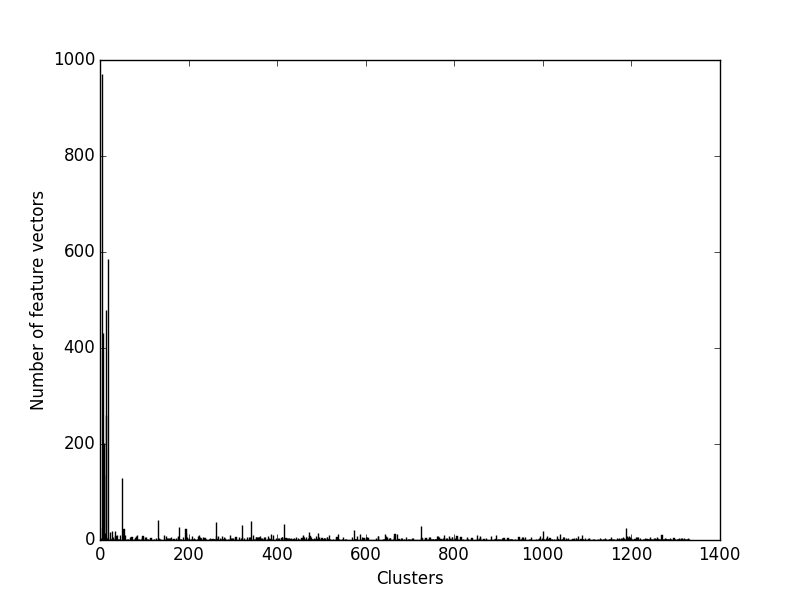
\includegraphics[width=0.6\textwidth]{./pythonScripts/pcaClustering.png}
      \caption{Clustering after PCA}
      \label{figure:pcaClustering}
\end{figure}
The performance measures show that the PCA dimensional reduction does not improve the quality of the clustering.\\\\
Given that the performance metrics are poor, the conclusion of this study is that the calculated feature vectors do not allow to differentiate between users.
\newpage
\label{subsection:kMeansStudy}
\subsection{Conclusion}
This section presented different explorations of the data. Feature vectors and data mining methods are explored in order to analyse student feedback activity on Music Circle and their academic performance.\\\\ 
Section \ref{subsection:differenceActivityFeedback} presents a method to construct feature vectors and visualise them. A five dimensional feature vector that contains feedback activity indicators is constructed. The visualisation in a video of all the feature vectors shows that in general feature vectors from different students are different, meaning that they can be used to differentiate between students.\\ Additionally, a difference matrix of the feature vectors is calculated. A heat map of the difference matrix is plotted confirming that the feature vectors can be used to make comparisons between students.\\\\ 
Section \ref{subsection:kNearestNeighbourStudy} presents a classification of students using $k$-nearest neighbour (KNN) algorithm. The feature vectors used to train the KNN algorithm are very similar to the previous ones but they add a new component measuring the total number of comments posted per user. In order to determine the optimal value of $k$, KNN is performed for $k$ between 2 $<=$ $k<=$ 80 and validated using cross-validation. The optimal performance of the algorithm is achieved using $k$=24 with an accuracy of 0.7980. Additional performance metrics calculated for $k$ = 24 are presented in Table \ref{table:performanceMetrics2}.
\newpage
\begin{table}[h]
	\centering
	\begin{tabular}{| l | l |}
		\hline
		 \textbf{Metric} & \textbf{Value} \\ \hline
		 Accuracy & 0.7980\\ \hline
		 Precision & 0.7300 \\ \hline
		 Recall & 0.8000 \\ \hline
		 F1 & 0.7600 \\ \hline
	\end{tabular}
	\caption{Performance metrics for the KNN classification}
	\label{table:performanceMetrics2}
\end{table}
\noindent The KNN performance values are high meaning that this method can accurately classify a student into a performance category using log data collected from an educational social network.\\\\
Section \ref{subsection:kMeansStudy} presents a fine resolution study of activity after feedback. Feature vectors are constructed considering activities on each session, therefore, each student has a set of feature vectors associated.\\
A data structure is constructed containing sets of feature vectors corresponding to different students and it is considered the ground truth. In order to prove that those sets can characterise students a $k$-Means clustering is proposed. The hypothesis is that if the sets of feature vectors characterise users a $k$-Means clustering algorithm with $k$ equal to the number of users will produce a similar clustering as the ground truth calculated. The performance metrics of the clustering process are poor, Table \ref{table:featureVectorsKMeans2} contains a summary of those metrics.
\begin{table}[h]
	\centering
	\begin{tabular}{| l | l |}
		\hline
		 \textbf{Metric} & \textbf{value} \\ \hline
		 Adjusted random index & 0.0004 \\ \hline
		 Adjusted mutual Information based scores & 0.0045 \\ \hline
		 Homogenity & 0.5380 \\ \hline
		 Completeness & 0.6433\\ \hline
		 V-measure & 0.5860\\ \hline
	\end{tabular}
	\caption{Examples of feature vectors}
	\label{table:featureVectorsKMeans2}
\end{table}
\noindent The performance of the $k$-Means clustering is poor. There is no difference between the clustering performed and a random clustering.\\
In order to try to improve the results a PCA is performed on the feature vectors. Table \ref{table:featureVectorsKMeansPCA2} shows the performance metrics of the clustering after the PCA dimensional reduction. Unfortunately, the results do not improve.
\begin{table}[h]
	\centering
	\begin{tabular}{| l | l |}
		\hline
		 \textbf{Metric} & \textbf{value} \\ \hline
		 Adjusted random index & 0.0012 \\ \hline
		 Adjusted mutual Information based scores & 0.0110 \\ \hline
		 Homogenity & 0.4799 \\ \hline
		 Completeness & 0.6299\\ \hline
		 V-measure & 0.5436\\ \hline
	\end{tabular}
	\caption{Examples of feature vectors}
	\label{table:featureVectorsKMeansPCA2}
\end{table}
The conclusion of this study is that the sets of feature vectors do not represent user behaviour and therefore are not valid to do student comparisons.
\label{conclusion}

\section{Self-reflection}
This section contains a self-reflection on the project as a whole. It contains a discussion about the difficulties encountered, as well as a summary of the results obtained and planned future work.\\\\
The initial project proposal considered to explore the fields of Data Mining, Machine Learning and Neural Networks to try to provide answers to questions about education. The data was to be obtained from an educational social network called Music Circle and it consisted in the students events log using the system. Machine learning algorithms were to be applied to this data. Additionally, it proposed to use Digital Signal Processing methods as a data analysis tool. Since the log events depend on time it was possible to construct a signal from the data.\\\\
The project explores how Data Mining can be applied to the dataset and it finds a method ($k$-Nearest Neighbour) that classifies students into academic performance with high accuracy. The Neural Network applications were not explored and the DSP perspective was only considered in the very early stages of the project. The main reason for not fulfilling completely the initial project proposal was a lack of time due to problems encountered setting the environment and also the difficulties in analysing the data. From the very beginning the complexities of the project manifested, these difficulties were both technical and theoretical.\\\\
The technical difficulties were related with setting up the development environment. Most of the technologies used were completely new to me, therefore, I had to learn about them. The development environment consisted in Python and Mongo running in a virtual environment \cite{VirtualEnv}. I chose to work in iPython notebooks because of its friendly IDE. However, iPython performance is bad when performing large printing operations which is a technique that I consider crucial for debugging. When iPython needs to print lots of messages on the console, it crashes and corrupts the file. Therefore, all the code is lost. After loosing a few of the scripts I decided to stop using iPython and run the Python scripts from the command line.\\ 
Another major difficulty in setting up the environment was to import the Research database. The importing process was slow and it took a lot of time to find a way to increase the computational speed. By using a Mongo distributed system the computational speed increased by at least a factor of 4. However, the learning and setting up of the Mongo distributed system was time consuming.\\\\
Once the environment was set up it was time to start the data analysis. The manipulation of the data was difficult due to their size and it was often complicated to test that the operations performed were correct. In this sense, a test driven development approach would have been helpful. Additionally, as with any real world dataset the data contained noise and inconsistencies that needed to be removed. This caused bugs and anomalous results that were often difficult to debug.\\\\
The theoretical problems were difficult to approach and they were related with research being at the core of this project. For example, it was clear to me what was the goal of the project but the exact path to achieve it was unclear. The time nature of the data made it difficult to manage, especially in the case of considering activity after feedback. One of the unresolved questions in this project is to determine when the consequences of feedback start and end. I made the assumption that the activity on each session was the result of an initial feedback event at the start of that session. This assumption simplified the problem but it did not solve it. In order to find a solution I should have found a differentiation between common activities and those that initiate and finalise feedback, this is a difficult task.\\\\
Four studies on the data are presented. Section \ref{section:statisticsStudy} explores the data in the Music Circle and Research database by building plots of the system activity over time and calculating statistics. In particular, linear regressions are fitted into the data, the results of the linear fitting are summarised in Table \ref{table:initialStudyResults2}. The value of the coefficient of determination ($r^2$) is low which indicates that the lines do not fit the data well.
\begin{table}[h]
	\centering
	\begin{tabular}{| l | l |}
		\hline
		 \textbf{Activity} & \textbf{$r^2$} \\ \hline
		 Uploads & 0.5067 \\ \hline
		 Comments views & 0.1576 \\ \hline
		 Owned tracks views & 0.1211 \\ \hline
		 Community tracks views & 0.1034 \\ \hline
		 Plays & 0.1154 \\ \hline
		 Comments posted & 0.1364 \\ \hline
	\end{tabular}
	\caption{Results of linear regressions on the different statistics}
	\label{table:initialStudyResults2}
\end{table}
\noindent \\Section \ref{section:exploratoryDataAnalysis} presents a deeper analysis of the data by constructing different feature vectors and applying Data Mining techniques to the student classification problem. The method to build the feature vectors consisted in cumulative measures of feedback activity, a technique suggested by Maia's paper \cite{Maia2008}. Sections \ref{subsection:differenceActivityFeedback} and \ref{subsection:kNearestNeighbourStudy} consider feature vectors built over the whole length of the case study yielding one feature vector per user. On section \ref{subsection:differenceActivityFeedback} methods that explore the ability of the feature vectors in differentiating users are explored. On section \ref{subsection:kNearestNeighbourStudy} a method to classify students into three classes of performance is explored. It trains a $k$-Nearest Neighbour algorithm to classify student performance into three categories from feature vectors that contain feedback activity indicators. The algorithm is validated using cross-validation, producing an accuracy of 0.7980. Table \ref{table:performanceMetrics} summarises the performance metrics of the algorithm.
\begin{table}[h]
	\centering
	\begin{tabular}{| l | l |}
		\hline
		 \textbf{Metric} & \textbf{Value} \\ \hline
		 Accuracy & 0.7980\\ \hline
		 Precision & 0.7300 \\ \hline
		 Recall & 0.8000 \\ \hline
		 F1 & 0.7600 \\ \hline
	\end{tabular}
	\caption{Performance metrics for the KNN classification}
	\label{table:performanceMetrics}
\end{table}
\noindent \\Section \ref{subsection:kMeansStudy} considers a higher resolution analysis of the data. The method to build the feature vectors considers the length of sessions yielding one feature vector per session. Therefore, each user has associated a set of feature vectors that contain feedback activity on the different sessions. A method to test how well the sets of feature vectors represents users is presented. All the feature vectors are fed into a $k$-Means clustering algorithm with $k$ = total number of users. The hypothesis made is that if the sets of feature vectors represent users, then the $k$-Means algorithm will produce clusters that are similar to the sets of feature vectors calculated. Table \ref{table:featureVectorsKMeans} presents the results. The clustering produced is similar to a random cluster, therefore, the conclusion is that the set of feature vectors are not useful in representing users.\\
In order to try to improve the results, a PCA dimensional reduction is performed and the same clustering method applied. The results are shown in Table \ref{table:featureVectorsKMeansPCA}, again the clustering algorithm is not able to produce a good clustering. This results indicate that the feature vectors calculated do not allow the differentiation of users.
\begin{table}[h!]
	\centering
	\begin{tabular}{| l | l |}
		\hline
		 \textbf{Metric} & \textbf{value} \\ \hline 
		 Adjusted random index & 0.0004 \\ \hline
		 Adjusted mutual Information based scores & 0.0045 \\ \hline
		 Homogenity & 0.5380 \\ \hline
		 Completeness & 0.6433\\ \hline
		 V-measure & 0.5860\\ \hline
	\end{tabular}
	\caption{Clustering performance metrics}
	\label{table:featureVectorsKMeans}
\end{table}
\begin{table}[h!]
	\centering
	\begin{tabular}{| l | l |}
		\hline
		 \textbf{Metric} & \textbf{value} \\ \hline
		 Adjusted random index & 0.0012 \\ \hline
		 Adjusted mutual Information based scores & 0.0110 \\ \hline
		 Homogenity & 0.4799 \\ \hline
		 Completeness & 0.6299\\ \hline
		 V-measure & 0.5436\\ \hline
	\end{tabular}
	\caption{Clustering performance metrics after PCA}
	\label{table:featureVectorsKMeansPCA}
\end{table}

\subsection{Future Work}
The future work is focused on fully exploiting the data and the techniques exposed in this report.\\
The data from the Coursera database was not fully explored. Particularly, the grades from the multiple choice questionnaire were not used. This data provides a rich insight in the learning process of students. Moreover, it can be used to track the learning process and measure the contribution of feedback on that learning.\\\\
In this project, only two Data Mining algorithms were used which is a low number given the variety of algorithms in the machine learning field. Neural Networks seem to have a lot of potential because of their ability to model highly complex data.\\\\
Feature vectors are the most important element in this project. They distil important information about students and allow the Data Mining algorithms to produce useful results. New feature vectors that consider the frequency of events instead of the number of them are of special interest. Such feature vectors would allow to remove the explicit dependancy on time which might allow for better comparisons between users. Additionally, this approach allows us to think about the spectrum of student behaviour which relates to the DSP approach exposed in the project proposal.


% More data mining algorithms
% contribution of feedback to the final grade
% Parts of the Coursera data are not explored

\bibliography{main}

\newpage
\appendix

\section{Code}
\subsection{Build the research database (by Chris Kiefer)}
	\lstinputlisting[language=Python]{./pythonScripts/importer.py}
	\label{importScript}
\subsection{Build the research database}
	\lstinputlisting[language=Python]{./pythonScripts/importShard1.py}
	\label{importShard1}
\subsection{Build the research database}
	\lstinputlisting[language=Python]{./pythonScripts/importShard2.py}
	\label{importShard2}
\subsection{Build the research database}
	\lstinputlisting[language=Python]{./pythonScripts/importShard3.py}
	\label{importShard3}
\subsection{Build the research database}
	\lstinputlisting[language=Python]{./pythonScripts/importShard4.py}
	\label{importShard4}
\subsection{Plot activities per day}
	\lstinputlisting[language=Python]{./pythonScripts/initialPerDayPlots.py}
	\label{initialPerDayPlots}
\subsection{Remove duplicates from activities array}
	\lstinputlisting[language=Python]{./pythonScripts/removeDuplicates.py}
	\label{removeDuplicates}

\subsection{Histogram of the feature vectors for all users}
	\lstinputlisting[language=Python]{./pythonScripts/generateHistogramsNoSessions.py}
	\label{featureVectorsHistograms}	

\subsection{Build feature vectors}
	\lstinputlisting[language=Python]{./pythonScripts/featureMatrix.py}
	\label{featureVectorsNoSessions}	
\subsection{Build the distance matrix}
	\lstinputlisting[language=Python]{./pythonScripts/distanceMatrix.py}
	\label{distanceMatrix}	
\subsection{Build a heat plot of the distance matrix}
	\lstinputlisting[language=Python]{./pythonScripts/heatPlot.py}
	\label{heatPlot}
\subsection{Add total number of activities and uploads for each user}
	\lstinputlisting[language=Python]{./pythonScripts/countUploadsAndActivities.py}
	\label{countActivitiesAndUploads}
\subsection{Import sessions for each user}
	\lstinputlisting[language=Python]{./pythonScripts/makeSessions.py}
	\label{makeSessions}
\subsection{Build the feature vectors}
	\lstinputlisting[language=Python]{./pythonScripts/featureVectorsToJson.py}
	\label{featureVectorsToJson}
\subsection{Link between Research and Coursera databases}
	\lstinputlisting[language=Python]{./pythonScripts/dbLink.py}
	\label{dbLink}
\subsection{Generate plots that compare general activity to grades achieved}
	\lstinputlisting[language=Python]{./pythonScripts/groundTruth.py}
	\label{groundTruth}
\subsection{Train and classify students with KNN}
	\lstinputlisting[language=Python]{./pythonScripts/kNearestNeighbour.py}
	\label{knn}
\subsection{Clustering the feature vectors}
	\lstinputlisting[language=Python]{./pythonScripts/clusteringFeatureSessionVectors.py}
	\label{clustering}
\subsection{Comparison of two clusters}
	\lstinputlisting[language=Python]{./pythonScripts/validateClusteringFeatureSessionVectors.py}
	\label{clusteringComparison}
\subsection{Comparison of two clusters}
	\lstinputlisting[language=Python]{./pythonScripts/pca.py}
	\label{script:pcaScript}

\section{Project proposal}
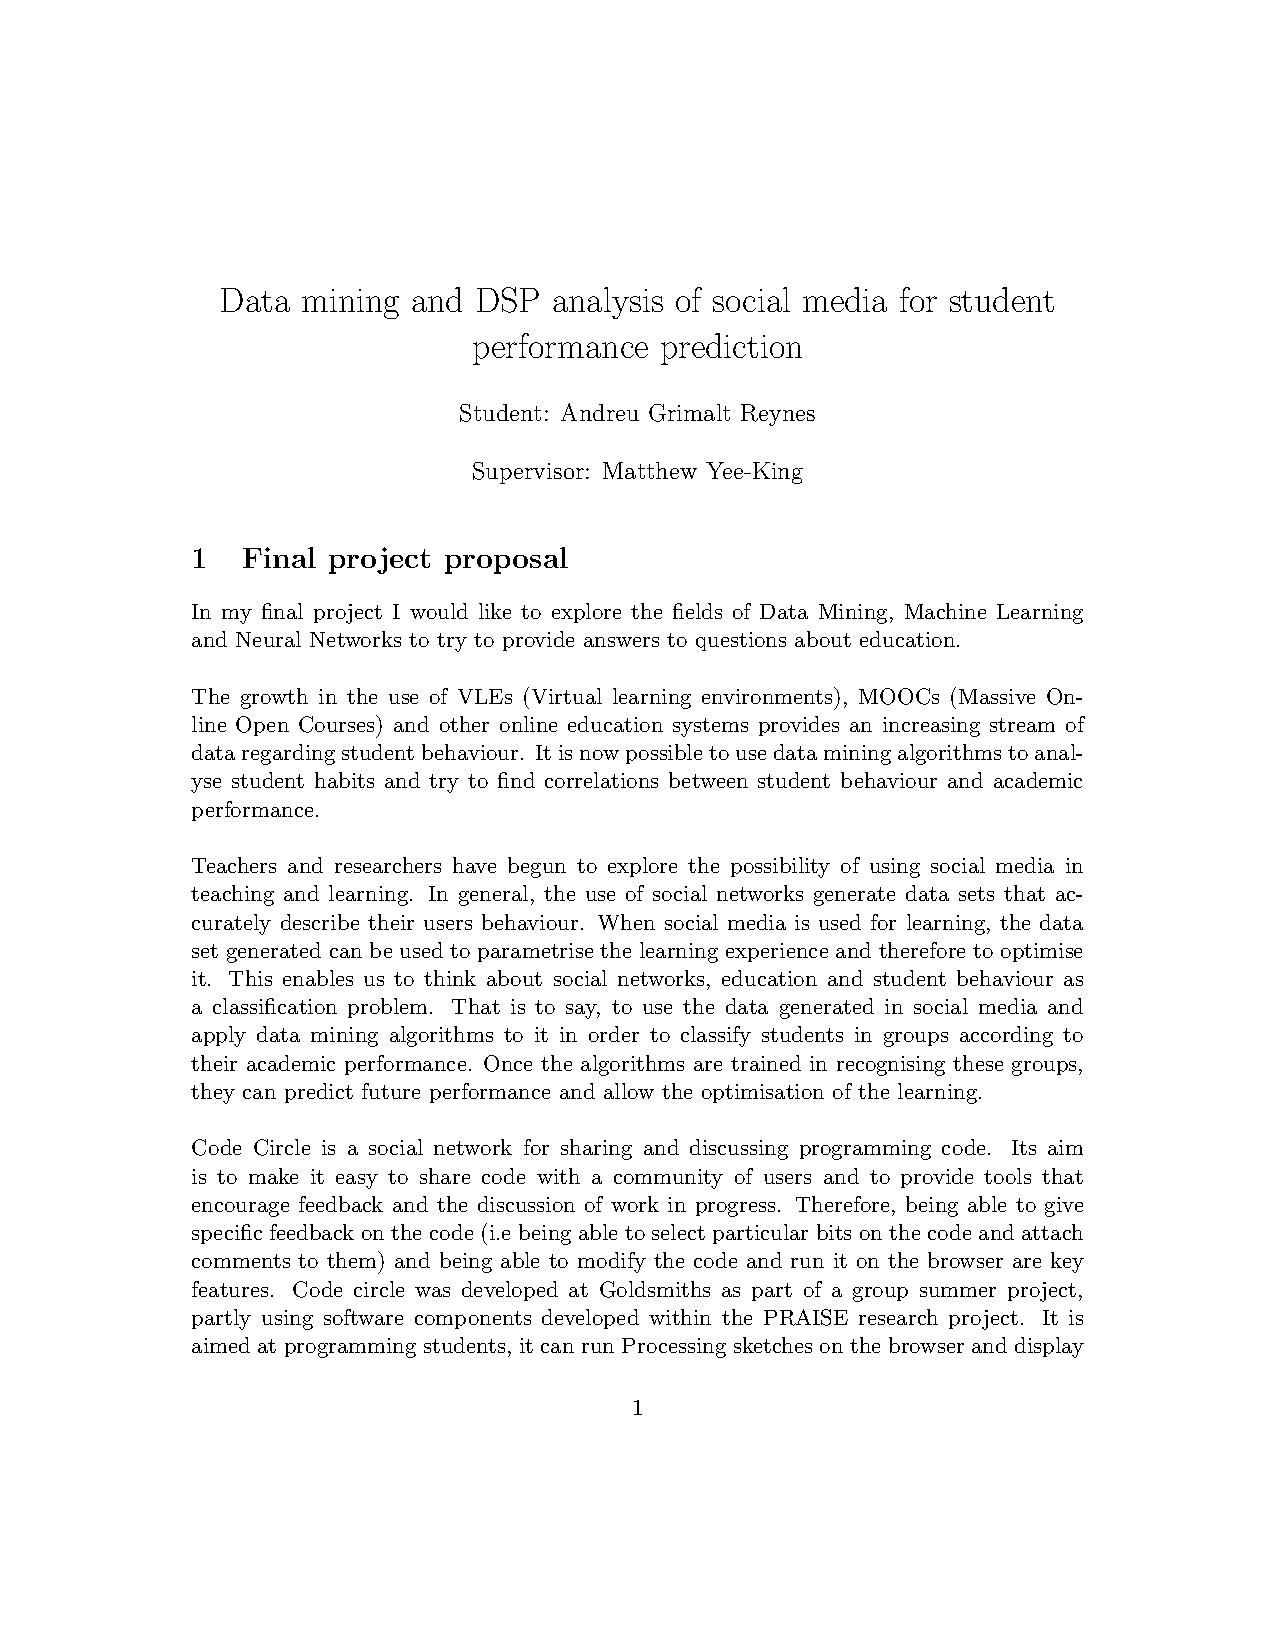
\includepdf[pages=-]{initial.pdf}

\section{Project preliminary report}
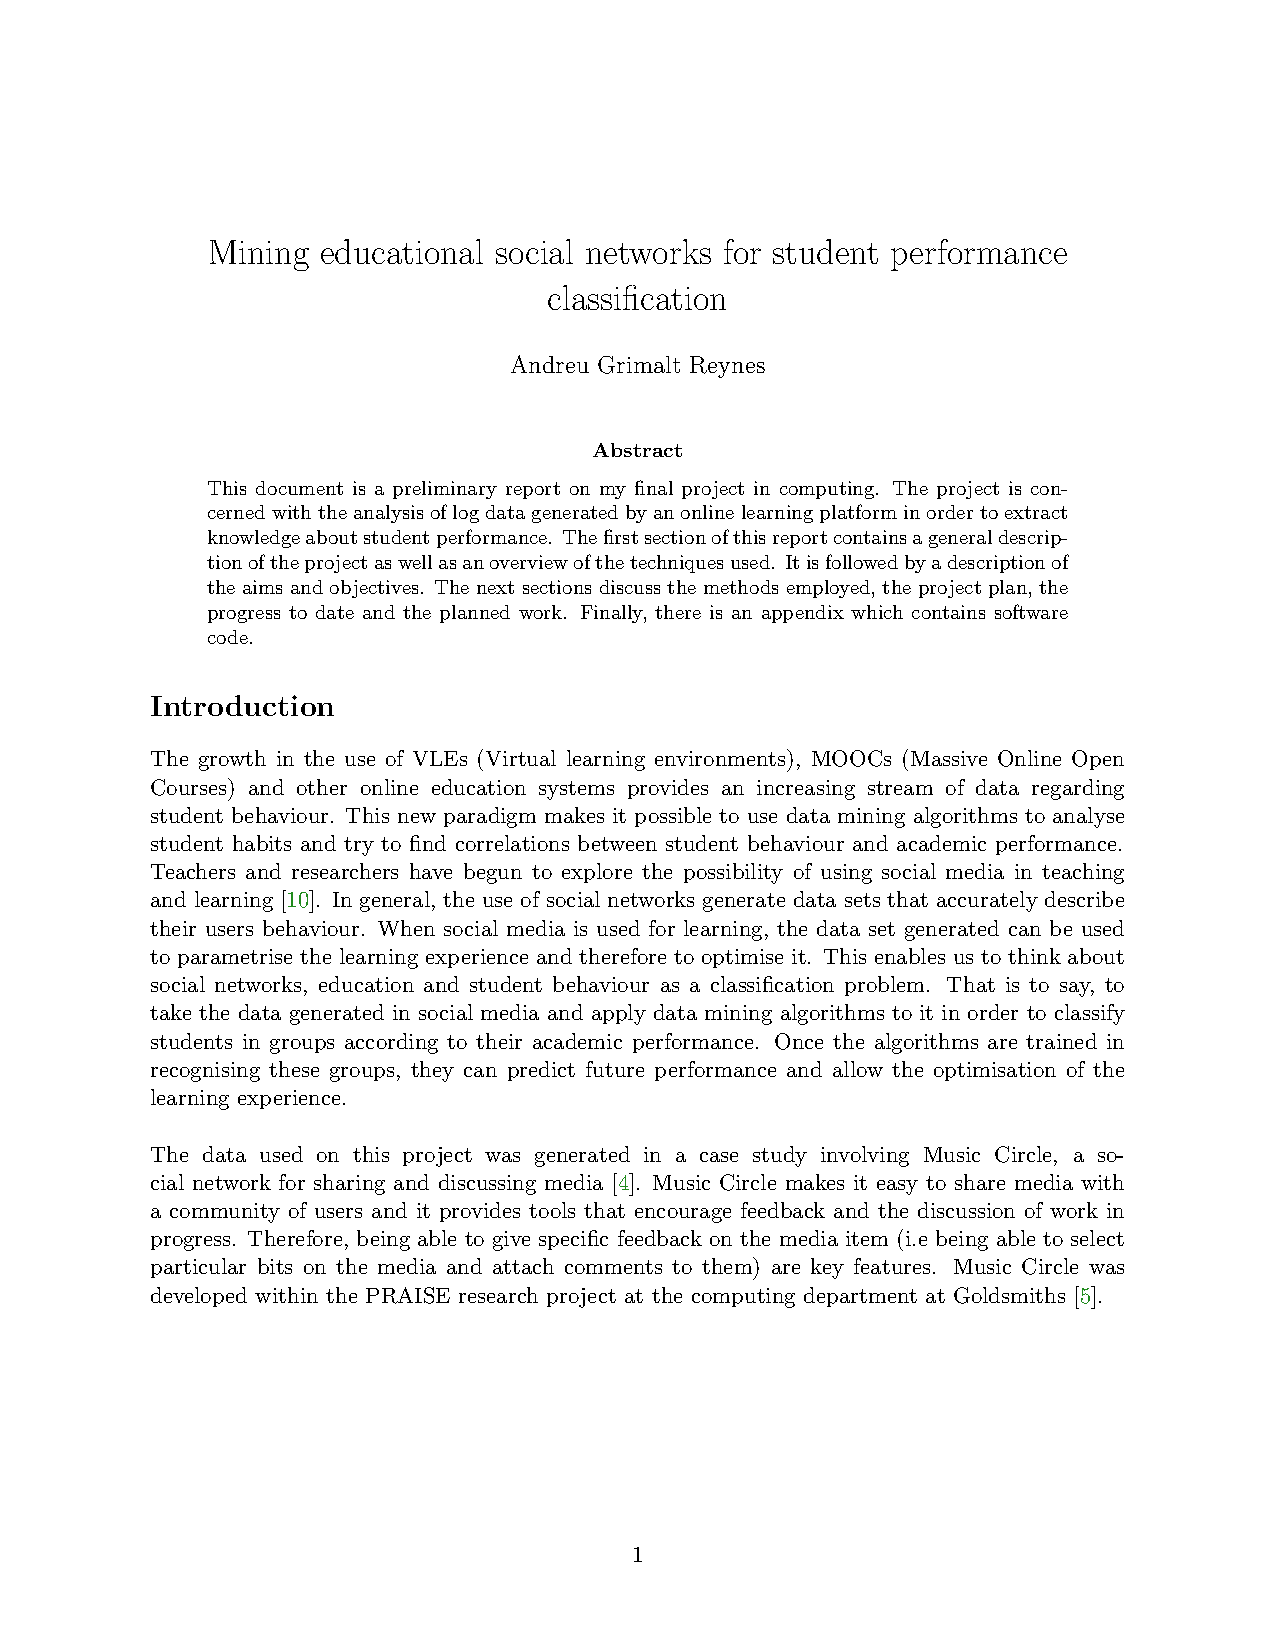
\includepdf[pages=-]{preliminaryReport.pdf}

\section{Weekly logs}
\subsection{19 January - 23 January}
\begin{tabularx}{\linewidth}{|X|X|}
  \hline
  Task & Notes \\
  \hline
  Set up GIT & Done \\
  \hline
  Set up python env & Done \\
  \hline
  Find if Basecamp is appropriate tool for printing all the tasks as I want to put that on the report & Will do the job as a list of todos. Ask Matthew if I can have a separate project on Basecamp \\
  \hline
  Start Python tests. Check Pymongo, Lists, Pylab (plots) & Done \\
  \hline
  Plot some simple statistics & Done \\
  \hline
  Check machine learning library & Planning to use scikit-learn\\
  \hline
  Did some FFT tests & Just to clarify concepts \\
  \hline
  Started thinking about DSP approach & Problems: are signals periodic? Check DSP approach on stock markets/economics \\
  \hline
  Arranged a meeting with Ben (PhD doing research on social networks) & Wednesday 28, 5:30, 329 \\
  \hline
\end{tabularx}

\subsection{2 February - 8 February}
\begin{tabularx}{\linewidth}{|X|X|X|}
  \hline
  Task & Notes & Hours \\
  \hline
  Check the log data generated & The data is valid from 30th of June & 24 \\
  \hline
  Problem: Log collection is huge & Made a cluster to speed up & 48\\
  \hline
  Check how other's use feature vectors & Read Baker's paper. They use feature vectors, summary here: https://basecamp.com/ 2065604/projects/ 1534650/todos/151387616 & 4 \\
  \hline
  Read `Towards sensor free affect detection in cognitive tutor algebra' & Summary here: https://basecamp.com/ 2065604/projects/ 1534650/todos/154618637 & 4 \\
  \hline
\end{tabularx}

\subsection{9 February - 15 February}
\begin{tabularx}{\linewidth}{|X|X|X|}
  \hline
  Task & Notes & Hours \\
  \hline
  Import research database & Set up sharded cluster, quite difficult & 40 \\
  \hline
  Try clustering on feature vectors & First you need to make them! & 16 \\
  \hline
\end{tabularx}

\subsection{16 February - 22 February}
\begin{tabularx}{\linewidth}{|X|X|X|}
  \hline
  Task & Notes & Hours \\
  \hline
  Wrote the preliminary report & Done & 40 \\
  \hline
\end{tabularx}

\subsection{23 February - 1 March}
\begin{tabularx}{\linewidth}{|X|X|X|}
  \hline
  Task & Notes & Hours \\
  \hline
  I did research on how people analyse social network data & I found papers that use feature vectors to find student academic performance from their activity in forums & 8 \\
  \hline
  I started to build the bibliography & Done & 2 \\
  \hline
  Coding & No progress so far. Finding it difficult to build the feature vectors. Also, iPython is really bad at printing and crashes a lot & 30 \\
  \hline
\end{tabularx}

\subsection{2 March - 8 March}
\begin{tabularx}{\linewidth}{|X|X|X|}
  \hline
  Task & Notes & Hours \\
  \hline
  Coding & Built feature vectors & 8 \\
  \hline
  Coding & Made histograms of feature vectors & 8 \\
  \hline
  Coding & Made a video with the histograms of the feature vectors, wrote a bit about it & 8 \\
  \hline
  Coding & Made a difference matrix with the feature vector, wrote a bit about it & 8 \\
  \hline
\end{tabularx}

\subsection{16 March - 22 March}
\begin{tabularx}{\linewidth}{|X|X|X|}
  \hline
  Task & Notes & Hours \\
  \hline
  Coding & Built new feature vectors that consider user sessions & 10 \\
  \hline
  Thought about clustering the feature vectors & Started trying clustering on feature vectors & 20 \\
  \hline
\end{tabularx}

\subsection{23 March - 29 March}
\begin{tabularx}{\linewidth}{|X|X|X|}
  \hline
  Task & Notes & Hours \\
  \hline
  Coding & Clustered the feature vectors & 10 \\
  \hline
  Research in how can I compare two clusters & Started trying clustering on feature vectors & 4 \\
  \hline
  Research in how to proceed once the clusters had been validated & I can calculate vector distribution in the clusters and then compare using Earth's moving distance & 16 \\
  \hline
\end{tabularx}

\subsection{30 March - 12 April}
\begin{tabularx}{\linewidth}{|X|X|X|}
  \hline
  Task & Notes & Hours \\
  \hline
  Write project report & - & - \\
   \hline
\end{tabularx}

\subsection{12 April - 26 April}
\begin{tabularx}{\linewidth}{|X|X|X|}
  \hline
  Task & Notes & Hours \\
  \hline
  Methods section on the report looking a bit weak, need to do another study on the data & Thinking about applying another DM algorithm to the data & - \\
   \hline
\end{tabularx}


\end{document}  










